\documentclass[a4paper,12pt]{article}

% убираю ворнинги
% \usepackage{silence}
% Уничтожаем ворнинги
% \WarningsOff*

\usepackage{cmap}
\usepackage{amssymb}
\usepackage{amsmath}
\usepackage{amsthm}
\usepackage[T2A]{fontenc}
\usepackage[utf8]{inputenc}
\usepackage[russian]{babel}
\usepackage{indentfirst}
\usepackage{epigraph}
\usepackage{extarrows}
\usepackage{framed}
\renewcommand{\epigraphsize}{\small}
\usepackage{relsize}
\usepackage{siunitx}
\usepackage{multicol}
\usepackage{enumitem}
\usepackage{stackengine,scalerel}
\def\dclesize{\ThisStyle{\raisebox{-.7pt}{\scalebox{1.45}{$\SavedStyle\bigcirc$}}}}
\def\dcle{\ensurestackMath{\stackon[0pt]{\leqslant}{\dclesize}}}
\def\cleq{\def\stacktype{L}\mathbin{\scalerel*{\dcle}{\dclesize}}}
% \pagestyle{empty}

\usepackage[left=1.25cm,right=1.25cm,
top=1.75cm,bottom=1.75cm]{geometry}
\usepackage{graphicx}
\graphicspath{ {./images/} }
\newcommand{\RomanNumeralCaps}[1] {\MakeUppercase{\romannumeral #1}}

\newcommand{\mysection}[2]{\setcounter{section}{#1}\addtocounter{section}{-1}\section{#2}}

% код
\DeclareRobustCommand{\svdots}{% s for `scaling'
\, \vcenter{%
\offinterlineskip
\hbox{.}
\vskip0.25\normalbaselineskip
\hbox{.}
\vskip0.25\normalbaselineskip
\hbox{.}%
}%
\,
}
\usepackage{listings}
\usepackage[unicode, pdftex]{hyperref}
\usepackage{xcolor}

\usepackage{dsfont}
\usepackage{mathabx}
\usepackage{multirow}
\usepackage{hhline}
\usepackage{float}

\usepackage{cancel}
\usepackage{breqn}

\usepackage{wrapfig}
\usepackage{stmaryrd}
\usepackage{mathrsfs}

\definecolor{linkcolor}{HTML}{50006b} % цвет ссылок
%\definecolor{urlcolor}{HTML}{107896} % цвет гиперссылок
\definecolor{urlcolor}{HTML}{50006b} % цвет гиперссылок
 
\hypersetup{pdfstartview=FitH,  linkcolor=linkcolor,urlcolor=urlcolor, colorlinks=true}

\definecolor{codegreen}{rgb}{0,0.6,0}
\definecolor{codegray}{rgb}{0.5,0.5,0.5}
\definecolor{codepurple}{rgb}{0.58,0,0.82}
\definecolor{backcolour}{cmyk}{0,0,0,0.05}

\lstdefinestyle{mystyle}{
backgroundcolor=\color{backcolour},
commentstyle=\color{codegreen},
keywordstyle=\color{magenta},
numberstyle=\tiny\color{codegray},
stringstyle=\color{codepurple},
basicstyle=\ttfamily\footnotesize,
breakatwhitespace=false,
breaklines=true,
captionpos=b,
keepspaces=true,
numbers=left,
numbersep=5pt,
showspaces=false,
showstringspaces=false,
showtabs=false,
tabsize=2,
texcl=true
}
\lstset{extendedchars=\true, style=mystyle}

\usepackage[pages = some]{background}
\backgroundsetup{
	scale = 1,
	angle = 0,
	opacity = 1,
	contents = {
\includegraphics[height = \paperheight, keepaspectratio]{background.jpg}}}
	
% объявление новых макрокоманд
% \newcommand{\Def}{\textbf{Определение:} } please use \begin{definition}
% \newcommand{\Statement}{\textbf{Утверждение:} }  please use \begin{statement}
% \newcommand{\Lemma}{\textbf{Лемма:} } please use \begin{lemma}
% \newcommand{\Th}{\textbf{Теорема:} } please use \begin{theorem}
\newcommand{\Task}{\textbf{Задача:} }
\newcommand{\Solution}{\textbf{Решение:} }
\newcommand{\Example}{\textbf{Пример:} }
% \newcommand{\Note}{\textbf{Замечание:} } please use \begin{lemmanote}
% \newcommand{\Cor}{\textbf{Следствие:} } please use \begin{corollary}
\newcommand{\Vars}{\textbf{Введем обозначения:} } 
% \newcommand{\Proof}{$\blacktriangle$ } please use \begin{proof}
% \newcommand{\EndProof}{$\blacksquare$ } please use \end{proof}
\newcommand{\del}{\partial}
\newcommand{\probspace}{(\Omega,\: \F,\: P)}

\renewenvironment{leftbar}[2][\hsize]
{
    \def\FrameCommand
    {
        {\hspace{20pt}
        \color{gray}\vrule width 3pt}
        \hspace{0pt}
    }
    \MakeFramed{\hsize#1\advance\hsize-\width\FrameRestore}
}
{\endMakeFramed}

\newcommand{\norm}{\triangleleft}
\newcommand{\bnorm}{\triangleright}

\newcommand{\angles}[1]{\left\langle{#1}\right\rangle}
\newcommand{\abs}[1]{\left|{#1}\right|}
\newcommand{\brackets}[1]{\left({#1}\right)}

\newcommand{\N}{\mathbb{N}}
\newcommand{\Z}{\mathbb{Z}}
\newcommand{\R}{\mathbb{R}}
\newcommand{\F}{\mathcal{F}}
\newcommand{\B}{\mathcal{B}}
\newcommand{\G}{\mathcal{G}}
\renewcommand{\C}{\mathbb{C}}
\newcommand{\Pxi}{P_\xi}
\newcommand{\pxi}{p_\xi}
\DeclareMathOperator{\E}{\mathbb{E}}
\newcommand{\D} { {\mathbb{D}}}
\newcommand{\indep}{\perp \!\!\! \perp}
\newcommand{\Norm}{\mathcal{N}}

\newtheorem{theorem}{Теорема}[section]
\newtheorem{corollary}{Следствие}[theorem]
\newtheorem{lemma}[theorem]{Лемма}
\newtheorem{statement}[theorem]{Утверждение}
\newtheorem{lemmanote}[theorem]{Замечание}
\newtheorem{trait}[theorem]{Свойство}
\newtheorem{definition}[theorem]{Определение}
\newcommand{\blank}[1]{\hspace*{#1}}




\makeatletter
\renewcommand{\dddot}[1]{%
  {\mathop{\kern\z@#1}\limits^{\vbox to-1.4\ex@{\kern-\tw@\ex@
   \hbox{\normalfont ...}\vss}}}}
\renewcommand{\ddddot}[1]{%
  {\mathop{\kern\z@#1}\limits^{\vbox to-1.4\ex@{\kern-\tw@\ex@
   \hbox{\normalfont....}\vss}}}}
\makeatother

\newcommand{\charac}[2]{\varphi_{#1}\brackets{#2}} % Хар.функция от распределения с.в. от аргумента
\newcommand{\eps}{\varepsilon}




\begin{document}
% ================ ПЕРВАЯ СТРАНИЦА ==========================
    \thispagestyle{empty}
    \BgThispage
    \begin{center}
        \vspace*{4cm}

        \Huge
        \textbf{Теория Вероятностей} \\
        \textbf{4 семестр} \\
        % \textbf{Билеты} \\
        \textbf{Лектор: Жуковский М.Е.} \\
        \textbf{весна 2022} \\
        
        \vspace{7cm}
        \Large
        \textbf{Авторы билетов (лучшие котики):} \\
        \href{https://vk.com/spitsynn}{Спицын Николай} \\
        \href{https://vk.com/dimasav123}{Савичев Дмитрий} \\
        \href{https://vk.com/id165779384}{Подзорова Полина} \\
        \href{https://vk.com/poli.dobro}{Чубенко Полина} \\        
        \href{https://vk.com/meraklim}{Климанова Ирина} \\
        \href{https://vk.com/ulegor}{Сбродов Егор} \\
        \href{https://vk.com/aldrmv}{Дремов Александр} \\
        \href{https://vk.com/id153425653}{Колтаков Михаил} \\
        
    \end{center}

\newpage

\tableofcontents
\newpage

% ===================== НАЧАЛО ======================

\section{Вероятностное пространство (\texorpdfstring{\(\Omega\)}{Omega}, \texorpdfstring{\(\mathcal{F}\)}{F} , P). Свойства вероятности. Теорема о непрерывности в “нуле” вероятностной меры (б/д).}
\begin{figure}[H]
\centering

\includegraphics[width=0.9\textwidth]{sections/Polya/1.jpg}
\end{figure}
\begin{figure}[H]
\centering

\includegraphics[width=0.9\textwidth]{sections/Polya/2.jpg}
\end{figure}

\section{Условные вероятности. Формула полной вероятности. Формулы Байеса. Независимость событий.}
\begin{figure}[H]
\centering

\includegraphics[width=0.9\textwidth]{sections/Polya/3.jpg}
\end{figure}

\section{Вероятностные меры на (\texorpdfstring{\(\mathbb{R}, \mathcal{B}(\mathbb{R})\)}{R, B(R)}). Функция распределения вероятностной меры, ее свойства. Теорема о построении вероятностной меры на (\texorpdfstring{\(\mathbb{R}, \mathcal{B}(\mathbb{R})\)}{R, B(R)}) по функции распределения (б/д).}
\begin{figure}[H]
\centering

\includegraphics[width=0.9\textwidth]{sections/Polya/4.jpg}
\end{figure}

\section{Дискретные и абсолютно непрерывные распределения, плотность. Примеры.}
\begin{figure}[H]
\centering

\includegraphics[width=0.9\textwidth]{sections/Polya/5.jpg}
\end{figure}
\begin{figure}[H]
\centering
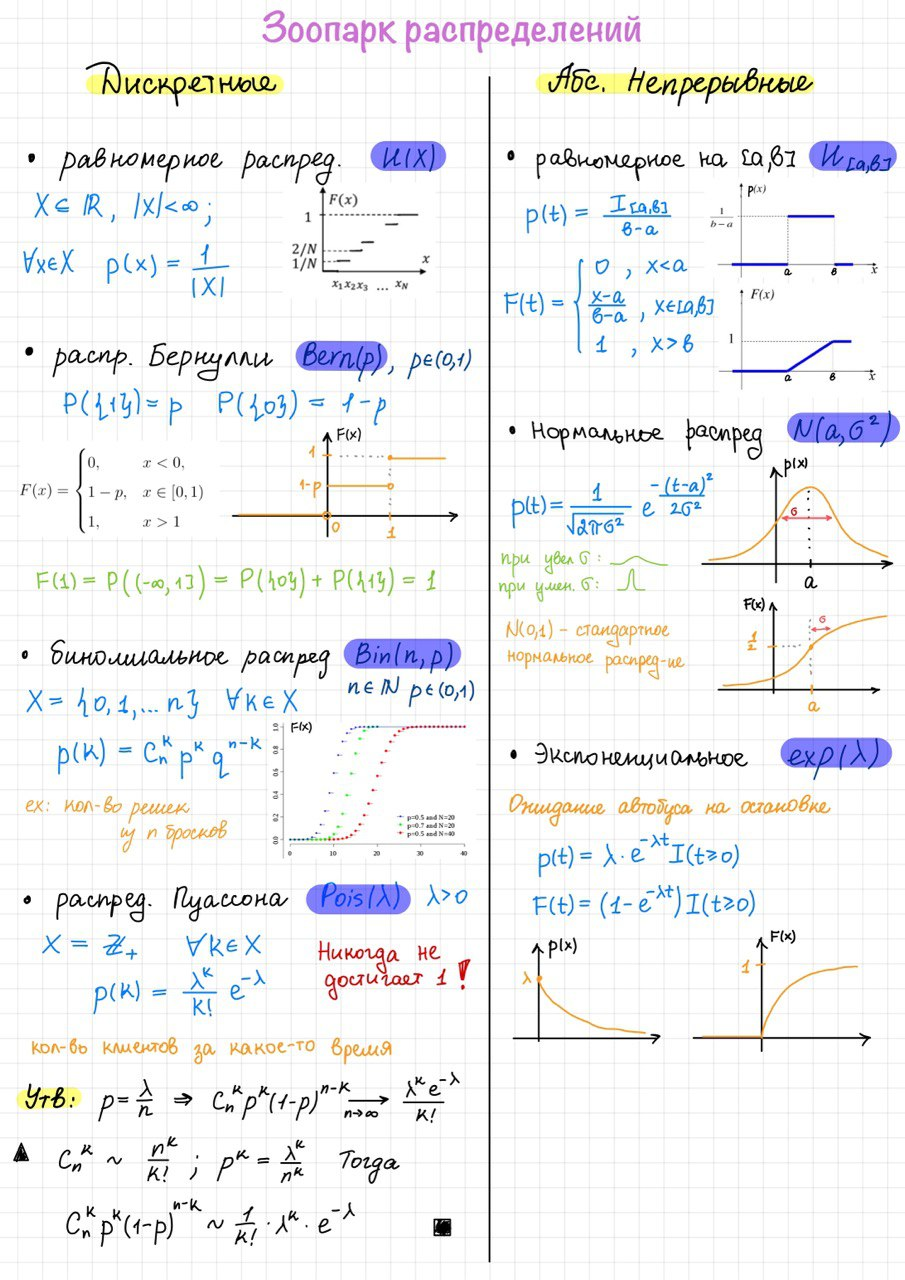
\includegraphics[width=0.9\textwidth]{sections/Polya/6.jpg}
\end{figure}

\section{Вероятностные меры на (\texorpdfstring{\(\mathbb{R}^n, \mathcal{B}(\mathbb{R}^n)\)}{R, B(R)}). Многомерная функция распределения, ее свойства. Теорема о построении вероятностной меры на (\texorpdfstring{\(\mathbb{R}, \mathcal{B}(\mathbb{R}^n)\)}{R, B(R^n)}) по функции распределения (б/д).}

\begin{definition}
Бореллевская сигма-алгебра на множестве $M$ --- наименьшая сигма-алгебра, содержащая все открытые подмножества (обознаяается $\B(M)$)
\end{definition}

\begin{definition}
Вероятность на $(\R^n, \B(\R^n))$ называется распределением вероятностей в $\R^n$.
\end{definition}

\begin{definition}
Функция распределения $F: \R^n \to [0, 1], \ F(x_1, \ldots, x_n) = P((-\infty, x_1] \times \ldots \times (-\infty, x_n])$
\end{definition}

\begin{statement}
Если $P_1, P_2$ -- распределения вероятностей с функциями распределения $F_1, F_2$ соответственно и $F_1 = F_2$, то $P_1 = P_2$.
\end{statement}

\textbf{Свойства:}

\begin{enumerate}
    \item $\forall a_1 \leqslant b_1, \ldots, a_n \leqslant b_n: \Delta_{a_1, b_1}^1 \ldots \Delta_{a_n, b_n}^n F(x_1, \ldots, x_n) \geqslant 0$, где $\Delta_{a_i, b_i}^i f(x_1, \ldots, x_n) = \newline = f(x_1, \ldots, x_{i-1}, b_i, x_{i + 1}, \ldots, x_n) - f(x_1, \ldots, x_{i-1}, a_i, x_{i+1}, \ldots, x_n)$
    
    По сути, мы хотим, чтобы вероятность параллелепипеда, натянутого на вершины 
    
    $(a_1, \ldots, a_n), (b_1, \ldots, b_n)$ был неотрицательным.
    
    \begin{proof}
    Индукцией по $k$ докажем, что $\Delta_{a_k, b_k}^k \ldots \Delta_{a_n, b_n}^n F(x_1, \ldots, x_n)  = P((-\infty, x_1] \times \ldots \times (-\infty, x_{k-1}] \times (a_k, b_k] \times \ldots \times(a_n, b_n])$
    
    \textbf{База: $k = n$}
    
    $\Delta_{a_n, b_n}^n F(x_1, \ldots, x_n) = F(x_1, \ldots, x_{n-1}, b_n) - F(x_1, \ldots, x_{n-1}, a_n) = P((-\infty, x_1] \times \ldots \times (-\infty, x_{n-1}] \times(a_n, b_n])$
    
    
    \textbf{Переход (для $k$ утв. доказано, докажем для $k-1$):}
    
    $\Delta_{a_{k-1}, b_{k-1}}^{k-1} \ldots \Delta_{a_n, b_n}^n F(x_1, \ldots, x_n) = \Delta_{a_{k-1}, b_{k-1}}^{k-1} \ P((-\infty, x_1] \times \ldots \times (-\infty, x_{k-1}] \times (a_k, b_k] \times \ldots \times(a_n, b_n]) = P((-\infty, x_1] \times \ldots \times (-\infty, x_{k-2}] \times (-\infty, b_{k-1}] \times (a_k, b_k] \times \ldots \times(a_n, b_n]) - P((-\infty, x_1] \times \ldots \times (-\infty, x_{k-2}] \times (-\infty, a_{k-1}] \times (a_k, b_k] \times \ldots \times(a_n, b_n]) = P((-\infty, x_1] \times \ldots \times (-\infty, x_{k-1}] \times (a_k, b_k] \times \ldots \times(a_n, b_n])$
    
    В частности, при $k = 1 \ \Delta_{a_1, b_1}^1 \ldots \Delta_{a_n, b_n}^n F(x_1, \ldots, x_n) = P((a_1, b_1] \times \ldots \times(a_n, b_n]) \geqslant 0$
    
    \end{proof}
    
    \item Непрерывность справа. 
    
    \begin{definition}
    $y = (y_1, \ldots, y_n) \geqslant (x_1, \ldots, x_n) = x$, если $\forall i : y_i \geqslant x_i$
    \end{definition}
    
    \begin{definition}
    Последовательность $x^k$ (в данном случае $k$ --- верхний индекс) стремится к $x$ справа ($x^k \downarrow x$), если $\forall k : x^{k+1} \leqslant x^k$ и $x = \lim\limits_{k \to \infty} x^k$
    \end{definition}
    
    Теперь к самому свойству: $\forall x^k \downarrow x \ \!\! : \lim\limits_{k \to \infty} F(x^k) = F(x)$
    
    \begin{proof}
    \[\lim\limits_{k \to \infty}F(x^k) = \lim\limits_{k \to \infty}  P((-\infty, x_1^k] \times \ldots \times(-\infty, x_n^k]) = P\left(\bigcap\limits_{k} (-\infty, x_1^k] \times \ldots \times(-\infty, x_n^k])\right) =\]
    \[= P((-\infty, x_1] \times \ldots \times(-\infty, x_n]) = F(x)\]
    \end{proof}
    
    \item $\lim\limits_{x_1 \to \infty, \ldots, x_n \to \infty} F(x_1, \ldots, x_n) = 1$
    
    $\forall i : \lim\limits_{x_i \to -\infty} F(x_1, \ldots, x_n) = 0$
    
    \begin{proof}
    $\lim\limits_{x_1 \uparrow +\infty, \ldots, x_n \uparrow +\infty} F(x_1, \ldots, x_n) = \lim \ P((-\infty, x_1] \times \ldots \times(-\infty, x_n]) = P(\mathbb{R}^n) = 1$
    
    $\lim\limits_{x_i \downarrow -\infty}\!\! F(x_1\ldots, x_n) \!=\! P((-\infty, x_1] \!\times \ldots \times\! (-\infty, x_{i-1}] \!\times\! \varnothing \!\times\! (-\infty, x_{i+1}] \times \ldots \times (-\infty, x_n]) \!=\! P(\varnothing) \!=\! 0$
    \end{proof}
\end{enumerate}

\begin{theorem}
Если $F\!\!: \R^n \to [0, 1]$ обладает свойствами $1)-3)$, то найдётся рапределение вероятностей, для которого $F$ --- функция распределения (б/д)
\end{theorem}


\section{Маргинальные распределения. Дискретные и абсолютно непрерывные многомерные распределения, плотность.}

\textbf{Маргинальные распределения}

\begin{definition}
Пусть $P$ -- распределение на $(\mathbb{R}^n, B(\mathbb{R}^n)), i \in \{1, \ldots, n\}, B \in B(\mathbb{R})$
\end{definition}

Тогда $P_i(B) = P(\R^{i-1} \times B \times \R^{n-i})$ -- распределение на $(\R, B(\R))$. Оно называется \textit{маргинальным}. (Идейно -- что-то вроде проекции на оси)

Довольно просто проверить корректность определения (что это действительно распределение).

По маргинальным распределениям можно построить многомерное (не единственным образом, однако, каким-то можно).

Наиболее естественный такой:
 
Пусть $P_1, \ldots, P_n$ -- распределения на $(\R, B(\R))$. Положим $P(B_1 \times \ldots \times B_n) = P_1(B_1) \cdot \ldots \cdot P_n(B_n)$ -- \textit{декартово произведение распределений} $P_1, \ldots, P_n$. У него $F(x_1, \ldots, x_n) = F_1(x_1) \cdots \ldots \cdot F_n(x_n)$.
 
\begin{lemmanote} 
Это распределение достаточно задать на декартовых произведениях борелевских множеств, дальше оно однозначно продолжится на всю сигма-алгебру. Более того, на самом деле, нам даже достаточно задать на декартовых произведениях лучей (потому что, как мы знаем, лучами можно задать всю борелевскую сигма-алгебру на $\R$)\\
\end{lemmanote}


\textbf{Дискретные распределения}

Тут все аналогично одномерному случаю (примеры можно получить из одномерного с помощью декартова произведения).

$X \subset \R^n$ -- не более, чем счетное, $P(X) = 1 \Rightarrow P$ -- \textit{дискретное}

Теперь введем \textit{дискретную плотность} $p: X \to [0, 1], p(x) = P(\{x\})$

$\forall B \in B(\R^n) : P(B) = \sum\limits_{x \in X \cap B}p(x)$

\begin{lemmanote}
как и в одномерном случае, дискретное распределение можно задать, задав его значение в каждой точке. Оно будет единственным образом восстанавливаться из такого описания.\\
\end{lemmanote}

\textbf{Абсолютно непрерывное распределение}

\begin{definition}
Если $p: \R^n \to \R_+$ такова, что $\forall x \in \R^n$
\end{definition}

$F(x) = \int\limits_{-\infty}^{x_1}\ldots\int\limits_{-\infty}^{x_n} p(t_1, \ldots, t_n)dt_1\ldots dt_n$, то $P$ -- абсолютно непрерывное распределение с плотностью $p$.

\textbf{Свойства}

\begin{enumerate}
    \item $\forall B \in B(\R^n) : P(B) = \int\limits_B p dt_1\ldots dt_n$
    \item Если $p : \R^n \to \R_+, \int\limits_{\R^n}p dt_1 \ldots dt_n = 1$, то $p$ -- плотность некоторого распределения вероятностей
    \item Если $F$ дифференцируема по каждому аргументу, то $P$ -- абсолютно непрерывное распределение с плотностью $p(t_1, \ldots, t_n) = \frac{\partial^n F}{\partial t_1 \ldots \partial t_n}$
\end{enumerate}

Свойства 1) и 2) доказываются аналогично одномерной ситуации. Свойство 3) доказывается проверкой того, что интеграл плотности равен $F$, что, очевидно, верно.

\begin{statement}
Если $P_1, \ldots, P_n$ -- абсолютно непрерывные распределения на $(\R, B(\R))$ с плотностями $p_1, \ldots, p_n$, то $P_1 \times \ldots \times P_n$ -- абсолютно непрерывное распределение на $(\R^n, B(\R^n))$ с плотностью $p_1(t_1) \cdot \ldots \cdot p_n(t_n)$
\end{statement}

\begin{proof}
Положим $p(t_1, \ldots, t_n) = p_1(t_1) \cdot \ldots \cdot p_n(t_n)$. Проверим, что ее интеграл равен $F$:

$\int\limits_{-\infty}^{x_1}\ldots\int\limits_{-\infty}^{x_n} p(t_1, \ldots, t_n)dt_1\ldots dt_n = \int\limits_{-\infty}^{x_1}\ldots\int\limits_{-\infty}^{x_n}  p_1(t_1) \cdot \ldots \cdot p_n(t_n)dt_1\ldots dt_n = \int\limits_{-\infty}^{x_1}p_1(t_1)dt_1\ldots\int\limits_{-\infty}^{x_n}p_n(t_n)dt_n = F_1(x_1)\cdot \ldots \cdot F_n(x_n)$
\end{proof}

\begin{lemmanote}
дискретное распределение абсолютно непрерывно относительно считающей меры (в точках множества $M$ мера равна $1$, в остальных -- $0$)
\end{lemmanote}
\section{Измеримые отображения. Случайные величины и векторы. Критерий измеримости. Действия над случайными величинами и пределы последовательностей случайных величин.}

\begin{definition}
$(X, M) $ - \textit{измеримое пространство}, где $X$ --- единица, $M$ --- $\sigma$-алгебра. Элементы $M$ называются \textit{измеримыми множествами}
\end{definition} 

$(\Omega, \F, P)$ --- вероятностное пространство

$(E, \Sigma)$ --- измеримое пространство

\begin{definition}
\textit{Случайный элемент} $X: \Omega \to E$, причём, $(\F|\Sigma)$ --- измеримое.
\end{definition}

\begin{definition}
$X$ --- $(\F|\Sigma)$-измеримое $\Leftrightarrow \ [\forall B \in \Sigma : X^{-1}(B) \in \F]$

$P_X(B) := P(X \in B) := P(\{w : X(w) \in B\})$
\end{definition}

$P_X(B)$ --- вероятность на $(E, \Sigma)$

\begin{definition}
$P_X(B)$ называется \textit{распределением вероятностей $X$}\\

В частности,

\begin{itemize}
    \item если $E = \R, \Sigma = B(\R)$, то $X$ --- \textit{случайная величина},
    \item если $E = \R^n, \Sigma = B(\R^n)$, то $X$ --- \textit{случайный вектор}
\end{itemize}
\end{definition}

\begin{theorem}[Критерий измеримости]
Если $\mathcal{M} \subset \Sigma, \sigma(\mathcal{M}) = \Sigma$, то $X$ --- $(\F|\Sigma)$-измеримо $\Leftrightarrow \forall B \in \mathcal{M} : X^{-1}(B) \in \F$
\end{theorem}

(Доказательство критерия известно из октч --- его могут спросить на доп вопрос, в билете это б/д).

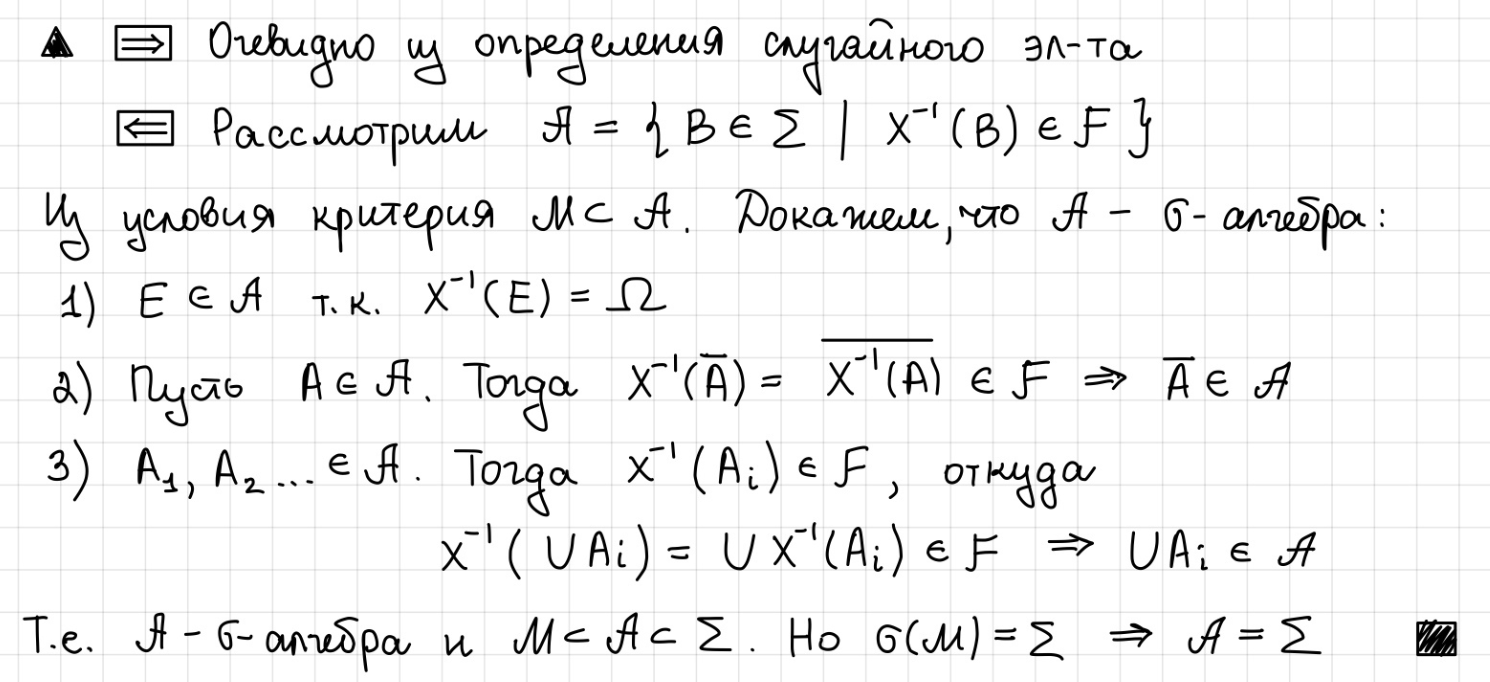
\includegraphics[scale=0.5]{images/izmerimost.png}

\begin{statement}
$\F_X = \{X^{-1}(B), B \in \Sigma\}$ --- $\sigma$-алгебра (порождённая $X$)
\end{statement}
\begin{proof}
\,\newline
\begin{enumerate}
    \item $X^{-1}(E) = \Omega \in \F_X$
    
    \item Если $A \in \F_X$, то $\exists B \in \Sigma$, что $X^{-1}(B) = A$
    
    $\overline{B} \in \Sigma \Rightarrow X^{-1}(\overline{B}) \in \F_X$. Но $X^{-1}(\overline{B}) = \overline{X^{-1}(B)} = \overline{A}$
    
    \item Если $A_1, A_2, \ldots \in \F_X$, то $\exists B_1, B_2, \ldots \in \Sigma: X^{-1}(B_i) = A_i$
    
    $\cup A_i = X^{-1}(\cup B_i) \in \F_X$ (т.к. $\cup B_i \in \Sigma$)
\end{enumerate}
\end{proof}

\textbf{Действия над случайными величинами}

\begin{definition}
$f: \R^n \to \R^k$ --- \textit{борелевская}, если $\forall B \in B(\R^k) : f^{-1}(B) \in B(\R^n)$
\end{definition}

\begin{theorem}
Пусть $\xi$ --- $n$-мерный случайный вектор, $\eta : \Omega \to \R^k$

Тогда $\eta $ --- $\F_{\xi}$-измеримый случайный вектор (то есть $\forall B \in B(\R^k) \eta^{-1}(B) \in F_{\xi}$) $\Leftrightarrow \exists$ борелевская функция $f : \R^n \to \R^k : \eta = f(\xi)$
\end{theorem}

Справа налево очевидно, слева направо оставил б/д.

\begin{statement}
$\xi = (\xi_1, \ldots, \xi_n)$ --- случайный вектор $\Leftrightarrow \xi_1, \ldots, \xi_n$ --- случайные величины.
\end{statement}

\begin{proof}
\:\newline
\begin{itemize}
    \item $i \in \{1, \ldots, n\}, B \in B(\R)$
    
    $\xi_i^{-1}(B) = \{w : \xi_i(w) \in B\} = \{w : \xi(w) \in \R^{i-1} \times B \times \R^{n-i}\} \in \F$
    
    Значит, $\xi_i$ -- случайная величина
    
    \item $\sigma(\{B_1 \times \ldots \times B_n\})=\B(\R^n)$
    
    $\xi^{-1}(B_1 \times \ldots \times B_n) = \{w : \xi(w) \in B_1 \times \ldots \times B_n\} = \{w : \xi_1(w) \in B_1, \ldots, \xi_n(w) \in B_n\} = \bigcap\limits_{i=1}^n \{w : \xi_i(w) \in B_i\} = \bigcap\limits_{i=1}^n \xi_i^{-1}(B_i) \in \F$
\end{itemize}
\end{proof}

\begin{statement}
Любая непрерывная (кусочно-непрерывная) функция является борелевской.
\end{statement}

\begin{corollary}
Если $\xi,\, \eta$ --- случайные величины, то $\xi + \eta,\, \xi - \eta,\, \xi \cdot \eta,\, \frac{\xi}{\eta} \cdot I(\eta \neq 0)$ --- случайные величины
\end{corollary}

\begin{statement}
Если $\xi_1,\, \xi_2,\, \ldots$ --- случайные величины, то $\inf\limits_{n} \xi_n,\: \sup\limits_{n} \xi_n,\: \underset{n \to \infty}{\underline{\text{lim}}} \xi_n,\: \underset{n \to \infty}{\overline{\text{lim}}} \xi_n$ --- случайные величины.
\end{statement}

\begin{proof}
\:\newline
\begin{enumerate}
    \item $\xi = \sup\limits_{n} \ \xi_n$
    
    $\xi^{-1}((-\infty, x]) = \{w: \xi(w) \leqslant x\} = \{w : \forall n \xi_n \leqslant x\} = \bigcap\limits_{n} \xi_n^{-1}((-\infty, x]) \in \F$
    
    \item $\xi = \inf\limits_{n} \ \xi_n$
    
    $\xi^{-1}([x, +\infty)) = \bigcap\limits_{n} \xi_n^{-1}([x, +\infty)) \in \F$
    
    \item $\xi = \underset{n \to \infty}{\overline{\text{lim}}} \xi_n$
    
    $\xi^{-1}((x, +\infty)) = \bigcup\limits_{\varepsilon > 0} \{w\!\!\! : \forall k \exists n \geqslant k \ \xi_n > x + \varepsilon\} = \bigcup\limits_{m \in N} \{w\!\!\! : \forall k \exists n \geqslant k \ \xi_n > x + \frac{1}{m}\} =$
    $= \bigcup\limits_{m}\bigcap\limits_{k}\bigcup\limits_{n \geqslant k} \left\{\xi_n > x + \frac{1}{m}\right\} \in \F$
    
    \item $\xi = \underset{n \to \infty}{\underline{\text{lim}}} \xi_n$
    
    $\xi^{-1}((-\infty, x)) = \bigcup\limits_{\varepsilon > 0} \{w : \forall k \exists n \geqslant k \ \xi_n < x - \varepsilon\} = \bigcup\limits_{m}\bigcap\limits_{k}\bigcup\limits_{n \geqslant k}\left\{\xi_n < x - \frac{1}{m}\right\} \in \F$
\end{enumerate}
\end{proof}

\section{Характеристики случайной величины (вектора): распределение вероятностей, функция распределения, плотность.}

\begin{definition}
Пусть $\xi$ -- случайный вектор, $P_{\xi}$ -- \textit{ распределение} $\xi$,  $P_{\xi} : B(\mathbb{R}^n) \to [0, 1] : P_{\xi}(B) = P(\{w : \xi(w) \in B\})$

$F_{\xi}: \mathbb{R}^n \to [0, 1]$ -- функция распределения, соответствующая $P_{\xi}$ -- \textit{функция распределения} $\xi$


Если $P_{\xi}$ дискретно, то $\xi$ -- \textit{дискретный случайный вектор}

Если $P_{\xi}$ абсолютно непрерывно, то $\xi$ -- \textit{абсолютно непрерывный случайный вектор}

Если $p_{\xi}$ -- плотность $P_{\xi}$, то $p_{\xi}$ -- \textit{плотность вектора $\xi$}
\end{definition}

\section{Независимость случайных величин. Независимость произвольного набора случайных величин. Критерий независимости, теорема о независимости борелевских функций от непересекающихся наборов независимых случайных величин. Напоминание формулировки теоремы Фуббини. Свёртка распределений.}
\begin{definition} Случайные вектора $\xi, \ \eta$ называются \textit{независимыми}, если
\[\forall B_1 \in \B(R^{k_1}), B_2 \in \B(R^{k_2}): \ P(\xi \in B_1, \eta \in B_2) = P(\xi \in B_1)P(\eta \in B_2)\]
\end{definition}

\begin{definition} Случайные вектора $\xi_1, \ldots , \xi_n$ называются \textit{независимыми}, если  \\ $\forall  B_1 \in \B(\R^{k_1}),\ldots ,  B_n \in \B(\R^{k_n})$ выполнено, что 
\[P(\xi_1 \in B_1, \ldots ,  \xi_n \in B_n) = P(\xi_1 \in B_1) \cdot \ldots  \cdot P(\xi_n \in B_n)\]
\end{definition}

\begin{definition}  $\{\xi_{\alpha} , \alpha \in \Gamma\}$ \textit{независимы}, если $\forall n \in \N  \ \forall \alpha_1, \ldots , \alpha_n \in \Gamma$ (попарно различных) $: \ \xi_{\alpha_1}, \ldots , \xi_{\alpha_n} $ независимы.
\end{definition}

\begin{definition}
Система множеств $\Sigma$ называется $\pi$-системой, если
\[\forall A, B \in \Sigma: A\cap B \in \Sigma\]
\end{definition}

\begin{definition}
Система множеств $\Sigma $ называется $\lambda$-системой, если 
\begin{itemize}
    \item[1.] $E \in \Sigma$
    \item[2.] $ A, B \in \Sigma, A \subset B: B \backslash A \in \Sigma$
    \item[3.] $A_1 \subset A_2\ldots   \in \Sigma: \ \bigcup\limits_{n} A_n \in \Sigma$
\end{itemize}
\end{definition}

\begin{lemma}[б/д]
Если $\Sigma - \pi$-система, то $\sigma(\Sigma) = \lambda(\Sigma)$ 
\end{lemma}


\begin{theorem}[Критерий независимости]
$\xi_1, \ldots , \xi_n$ --- независимые случайные величины тогда и только тогда когда 
\[\forall (x_1, \ldots , x_n) \in R^{n}\;\;  F_{(\xi_1, \ldots , \xi_n)}(x_1, \ldots , x_n) = F_{\xi_1}(x_1)\ldots  F_{\xi_n}(x_n).\]
В случае векторов:
\[\forall x_1 \in \R^{k_1}, \ldots  ,  x_n \in \R^{k_n}\;\; F_{(\xi_1, \ldots , \xi_n)}(x_1, \ldots , x_n) = F_{\xi_1}(x_1)\ldots F_{\xi_n}(x_n).\]
\begin{proof}
Проведем доказательство для случайных величин. В правую сторону утверждение очевидно, докажем в обратную. То есть равенство выполнено для лучей, а надо доказать для всех борелевских
множеств. Докажем по индукции, что
\[
    \forall k \in \{1, \ldots , n\} \ \forall B_1,\ldots , B_k \in \B(\R) \ \forall \ x_{k+1},\ldots , x_n \in \R
\]
\begin{multline*}
     P(\underbrace{\xi_1 \in B_1,\ldots , \xi_k \in B_k}_{k\text{ штук из }B_i},
     \underbrace{\xi_{k+1} \leqslant x_{k+1}, \ldots , \xi_n \leqslant x_n}_{\text{оставшиеся меньше } x_i}) = \\
     P(\xi_1 \in B_1) \ldots P(\xi_k \in B_k)P( \xi_{k+1} \leqslant x_{k+1}) \ldots  P(\xi_n \leqslant x_n).
\end{multline*}
База $k = 0$~--- тривиально. Пусть доказано для $k$. Хотим доказать для $k+1$.

Фиксируем $B_1, \ldots , B_k \in \B(\R), \ x_{k+2}, \ldots , x_n \in \R$
Рассмотрим 
\begin{multline*}
M = \{B \in \B(\R):\;P(\xi_1 \in B_1,\ldots, \xi_{k} \in B_k, \underline{\xi_{k+1} \in B},\xi_{k+2} \leqslant x_{k+2}, \ldots , \xi_n \leqslant x_n) =\\
 = P(\xi_1 \in B_1)\ldots P(\xi_k \in B_k)P(\xi_{k+1} \in B) P(\xi_{k+2} \leqslant x_{k+2})\ldots P(\xi_{n} \leqslant x_{n})\}.
\end{multline*}

Так как $(-\infty, x] \in M \implies \sigma(M) = \B(\R)$. Значит, если мы докажем, что $M$~--- сигма-алгебра, мы докажем утверждение.

Знаем, что  $\{(-\infty, x]\} \subset M$ это $\pi$-система, тогда если $M$~--- $\lambda$-система,
то $M$~--- $\sigma$-алгебра.
\begin{enumerate}
    \item $\R \in M$:
    \begin{multline*}
        P(\xi_1 \in B_1, \ldots , \xi_k \in B_k, \underline{\xi_{k+1} \in \R},\xi_{k+2} \leqslant x_{k+2} \ldots , \xi_n \leqslant x_n) =\\
        \lim_{x\to\infty} P(\xi_1 \in B_1, \ldots  \xi_k \in B_k, \xi_{k+1} \leqslant x,\xi_{k+2} \leqslant x_{k+2} \ldots , \xi_n \leqslant x_n) 
        \xlongequal[\text{предп. индукции}]{}\\
        \lim_{x\to\infty} P(\xi_1 \in B_1) \ldots  P(\xi_k \in B_k)P(\xi_{k+1} \leqslant x)P( \xi_{k+2} \leqslant x_{k+2}) \ldots P(\xi_n \leqslant x_n)
    \end{multline*}
     \item $A, B \in M, A \subset B$:
     \begin{multline*}
     P(\xi_1 \in B_1, \ldots  \xi_k \in B_k, \underline{\xi_{k+1} \in (B \backslash A)},\xi_{k+2} \leqslant x_{k+2} \ldots , \xi_n \leqslant x_n) \xlongequal[\text{разность}]{}\\
     P(\xi_1 \in B_1, \ldots  \xi_k \in B_k, \underline{\xi_{k+1} \in B},\xi_{k+2} \leqslant x_{k+2} \ldots , \xi_n \leqslant x_n) - \\
     P(\xi_1 \in B_1, \ldots  \xi_k \in B_k, \underline{\xi_{k+1} \in A},\xi_{k+2} \leqslant x_{k+2} \ldots , \xi_n \leqslant x_n) =
     \end{multline*}
     \vspace*{-10mm}
     \begin{multline*}
     = P(\xi_1 \in B_1) \ldots  P(\xi_k \in B_k)\underline{P(\xi_{k+1} \in B)}P( \xi_{k+2} \leqslant x_{k+2}) \ldots P(\xi_n \leqslant x_n) - \\
     P(\xi_1 \in B_1) \ldots  P(\xi_k \in B_k)\underline{P(\xi_{k+1} \in A)}P( \xi_{k+2} \leqslant x_{k+2}) \ldots P(\xi_n \leqslant x_n) = \\
     P(\xi_1 \in B_1) \ldots  P(\xi_k \in B_k)\underline{P(\xi_{k+1} \in B \backslash A)}P( \xi_{k+2} \leqslant x_{k+2}) \ldots P(\xi_n \leqslant x_n).
     \end{multline*}
     Откуда $B \backslash A \in M$.
     \item $A_1, A_2 \ldots \in M,\;\; A_1 \subset A_2 \subset \ldots,
     \;\; A =\bigcup\limits_{n}A_n$
     \begin{multline*}
     P(\xi_1 \in B_1, \ldots  \xi_k \in B_k, \underline{\xi_{k+1} \in A},\xi_{k+2} \leqslant x_{k+2} \ldots , \xi_n \leqslant x_n) =\\
     \lim_{m\to\infty} P(\xi_1 \in B_1, \ldots  \xi_k \in B_k, \underline{\xi_{k+1} \in A_m},\xi_{k+2} \leqslant x_{k+2} \ldots , \xi_n \leqslant x_n) =\\
     \lim_{m\to\infty} P(\xi_1 \in B_1) \ldots  P(\xi_k \in B_k)\underline{P(\xi_{k+1} \in A_m)}P( \xi_{k+2} \leqslant x_{k+2}) \ldots P(\xi_n \leqslant x_n) =\\
     P(\xi_1 \in B_1) \ldots  P(\xi_k \in B_k)\underline{P(\xi_{k+1} \in A)}P( \xi_{k+2} \leqslant x_{k+2}) \ldots P(\xi_n \leqslant x_n).
     \end{multline*}
     Откуда $A \in M$.
\end{enumerate}
Значит, $M$~--- $\lambda$-система, а значит $M = \B(\R)$.
Утверждение доказано по индукции. В частности, при $n=k$ 
\[\forall B_1,\ldots B_n \in \B(\R) \: P(\xi_1 \in B_1, \ldots  \xi_n \in B_n) = P(\xi_1 \in B_1) \ldots  P(\xi_n \in B_n).\]
\end{proof}
\end{theorem}
\begin{lemma}
Если $\xi_1, \ldots , \xi_n$ --- независимые случайные величины, то ($\xi_1, \ldots , \xi_{k_1}$), ($\xi_{k_1 +1}, \ldots , \xi_{k_2}$), \ldots --- независые случайные векторы (все индексы различны)
\end{lemma}
\begin{proof}
$F_{(\xi_1, \ldots , \xi_{k_1}), \ldots .}(\underset{dim = k_1}{x_1}, x_2, \ldots ) = F_{(\xi_1, \ldots ., \xi_n)}(t_1, \ldots , t_n) = F_{\xi_1}(t_1) \ldots F_{\xi_n}(t_n) = \\   F_{(\xi_1,\ldots , \xi_{k_1})}(x_1)\ldots F_{(\xi_{k_1 +1}, \ldots , \xi_{k_2})}(x_2)\ldots .$
\end{proof}
\begin{theorem}
Пусть $\xi_1, \ldots , \xi_k$ --- независимые случайные векторы. Пусть $f_1, \ldots , f_n$ --- борелевские. $f_i: \R^{n_i} \rightarrow \R^{m_i}$, где $n_i$ --- размерность $\xi_i$. Тогда $f(\xi_1), \ldots , f(\xi_k)$ --- независимые
\end{theorem}

\begin{proof}
$B_1 \in \B(\R^m_1), \ldots , B_k \in \B(\R^m_k). \ P(f_1(\xi_1) \in B_1, \ldots , f_k(\xi_k) \in B_k) =  P(\xi_1 \in f_1^{-1}(B_1), \ldots , \xi_k \in f_k^{-1}(B_k)) = P(\xi_1 \in f_1^{-1}(B_1)) \ldots P( \xi_k \in f_k^{-1}(B_k)) = P(f_1(\xi_1) \in B_1) \ldots P(f_k(\xi_k) \in B_k)$
\end{proof}

\begin{theorem}[Фубини]
Пусть ($\Omega_1 \times \Omega_2, \mathcal{F}_1\times\mathcal{F}_2, P_1\times P_2$) --- декартово произведение ($\Omega_1, \mathcal{F}_1, P_1$), ($\Omega_2, \mathcal{F}_2, P_2$). $\mathcal{F}_1\times\mathcal{F}_2 = \sigma(A_1\times A_2, A_1 \in \mathcal{F}_1, A_2 \in \mathcal{F}_2)$. $P_1\times P_2 (A_1\times A_2) = P_1(A_1)P_2(A_2)$. \\ 
Пусть $$\int\limits_{\Omega_1 \times\Omega_2} |\xi|d(P_1 \times P_2) < \infty$$ $\xi$ --- случайная величина. Тогда
$$\int\limits_{\Omega_1 \times\Omega_2} \xi d\left(P_1 \times P_2\right) = \int\limits_{\Omega_1}\left(\int\limits_{\Omega_2} \xi dP_2\right) dP_1 = \int\limits_{\Omega_2}\left(\int\limits_{\Omega_1} \xi d P_1\right) dP_2$$
\end{theorem}
\begin{theorem}[Свёртка]
\end{theorem}
Пусть $\xi_1, \xi_2$ --- независимые случайные величины.
 $$F_{\xi_1 + \xi_2}(x) = P(\xi_1 + \xi_2 \leqslant x) = P_{(\xi_1, \xi_2)}(\{(u,v): u+v \leqslant x\} = D) = \int\limits_{D}dP_{(\xi_1, \xi_2)} = \int\limits_{D}d(P_{\xi_1} \times P_{\xi_2}) =$$
 $$= \int\limits_{-\infty}^{\infty}\left(\int\limits_{-\infty}^{x-u}d P_{\xi_2}\right)d P_{\xi_1} =  \int\limits_{-\infty}^{\infty}F_{\xi_2}(x-u)d P_{\xi_1}$$ 
В частности, если  $\xi_1, \xi_2 $ --- абсолютно непрерывны с плотностями $p_1, p_2$, то $$F_{\xi_1 + \xi_2}(x) = \int\limits_{-\infty}^{\infty}F_{\xi_2}(x-u) p_{\xi_1}(u)du$$
Кроме того $$p_{\xi_1 + \xi_2}(x) = \int\limits_{-\infty}^{\infty}p_{\xi_2}(x-u)p_{\xi_1}(u)du$$ в силу того что
$$\int\limits_{-\infty}^{x} p_{\xi_1 + \xi_2}(t) dt = \int\limits_{-\infty}^{x}\left(\int\limits_{\R} p_{\xi_1}(t-u)p_{\xi_2}(u)du\right)dt = \int\limits_{\R}p_{\xi_2}(u)du\left( \int\limits_{-\infty}^{x}p_{\xi_1}(t-u) dt\right)$$ = $$\int\limits_{\R}p_{\xi_2}(u)du\left( \int\limits_{-\infty}^{x-u}p_{\xi_1}(y) dy\right) = \int\limits_{\R}p_{\xi_2}(u)F_{\xi_2}(x-u)du = F_{\xi_1 + \xi_2}(x)$$
\section{Математическое ожидание случайной величины: определение для произвольных случайных величин, дискретных и абсолютно непрерывных. Примеры. Основные свойства математического ожидания.}

Пусть \( (\Omega, \F, P) \)~--- вероятностное пространство, \(\xi:\; \Omega \rightarrow \mathbb{R}\)~--- случайная величина.

Определим матожидание 

\[\E \xi = \int_{\Omega} \xi dP \xlongequal[x = \xi(\omega)]{\text{теорема о замене переменных}} \int_{\mathbb{R}} x d\Pxi.\]

Причем если интеграла не существует, то не существует и мат. ожидания. Мат ожидание может быть бесконечным. Определим такие случаи.

Определим
\[ \xi = \xi^+ - \xi^-,\quad \xi^+ = \max{(\xi, 0)},\;\; \xi^- = \max{(-\xi, 0)}.\]

Тогда
\begin{itemize}
    \item \(\int{\xi^+ dP < \infty},\; \int{\xi^- dP < \infty} \implies |\E{\xi}| < \infty\)
    \item \(\int{\xi^+ dP = \infty},\; \int{\xi^- dP < \infty} \implies \E{\xi} = +\infty\)
    \item \(\int{\xi^+ dP < \infty},\; \int{\xi^- dP = \infty} \implies \E{\xi} = -\infty\)
\end{itemize}

\subsubsection*{Случай \texorpdfstring{$\xi$}{кси}~--- дискретная}
Тогда носитель $X$~--- не более чем счётный: \(\Pxi (X) = 1\). В таком случае
\[\E \xi = \sum_{x \in X} xP(\xi = x).\]

\subsubsection*{Примеры}

\begin{enumerate}
    \item \(\xi \sim Bern(p), \; \pxi(\{1\}) = p, \pxi(\{0\}) = 1 - p\).
    \[\E \xi = p.\]
    \item \(\xi \sim Bin(n, p), \; \pxi(\{k\}) = C^k_n p^k (1-p)^{n-k}\).
    \begin{align*}
        \E \xi &= \sum_{k = 0}^n {k C^k_n p^k (1-p)^{n-k}}\\
        &= \sum_{k = 0}^n {\frac{n!}{(k-1)! (n-k)!}p^k (1-p)^{n-k}} = np\sum_{k = 1}^n {C_{n-1}^{k-1} p^{k-1} (1-p)^{n-k}}\\
        &= np (p + (1-p))^{n-1} = np
    \end{align*}
    \item \(\xi \sim Pois(\lambda), \; \pxi (\{k\}) = \frac{\lambda^k e^{-\lambda}}{k!}, k \in \mathbb{Z_+}\).
    \begin{align*}
        \E \xi = \sum_{k = 0}^{\infty}{k \frac{\lambda^k e^{-\lambda}}{k!}} &= \sum_{k = 0}^{\infty}{ \frac{\lambda^k e^{-\lambda}}{(k-1)!}}\\
        &= \lambda e^{-\lambda} \sum_{k = 1}^{\infty} \frac{\lambda^{k-1}}{(k-1)!} = \lambda e^{-\lambda} e^{\lambda} = \lambda.
    \end{align*}
\end{enumerate}

\subsubsection*{Случай \texorpdfstring{$\xi$}{кси}~--- абсолютно непрерывная}
В этом случае
\[\E\xi = \int_{\R}x \pxi(x) dx.\]

\begin{statement}
Если \(g:\R \rightarrow \R\)~--- бореллевская и $\Pxi$~--- абсолютно непрерывна, то
\[\int g(x)d\Pxi = \int g(x) \pxi(x) dx.\]
\end{statement}

\begin{proof}
Рассмотрим случаи.
\begin{enumerate}
    \item Если индикатор $g(x) = I(x \in B),\; B \in \B(\R)$, то 
    \begin{align*}
        \int_{\R} g(x) d\Pxi = \int_{B}d\Pxi = \Pxi(B)
        = \int_{B}\pxi(x) dx = \int_{\R} g(x) \pxi(x) dx.
    \end{align*}
    \item Если простая функция \(g(x) = \sum_{i=1}^n g_i I(x \in B_i),\; B_i \in \B(\R)\), то
    \begin{align*}
        \int_{\R}g(x) d\Pxi = \sum_{i = 1}^n g_i \int_{\R}I(x \in B_i) d\Pxi = \sum_{i = 1}^n g_i  \int_{\R}I(x \in B_i) \pxi(x) dx = \int_{\R} g(x) \pxi(x) dx.
    \end{align*}
    \item Если $g \geqslant 0$, то существует последовательность простых функций \(0 \leqslant g_n,\; g_n\uparrow g\). В таком случае
    \begin{align*}
        \int_\R{g(x) d\Pxi} = \lim_{n \rightarrow \infty} \int_\R g_n(x) d\Pxi =  \lim_{n \rightarrow \infty} \int_\R g_n(x) \pxi(x) dx = \int_\R {g(x) \pxi(x) dx}
    \end{align*}
    \item Случай произвольной \(g = g^+ - g^-\):
    \begin{align*}
        \int g(x) d\Pxi &= \int g^+(x) d\Pxi - \int g^-(x) d\Pxi \\
        &= \int g^+(x)\pxi dx - \int g^-(x)\pxi dx \\
        &= \int g(x)\pxi dx
    \end{align*}
\end{enumerate}
\end{proof}

\subsubsection*{Примеры}
\noindent 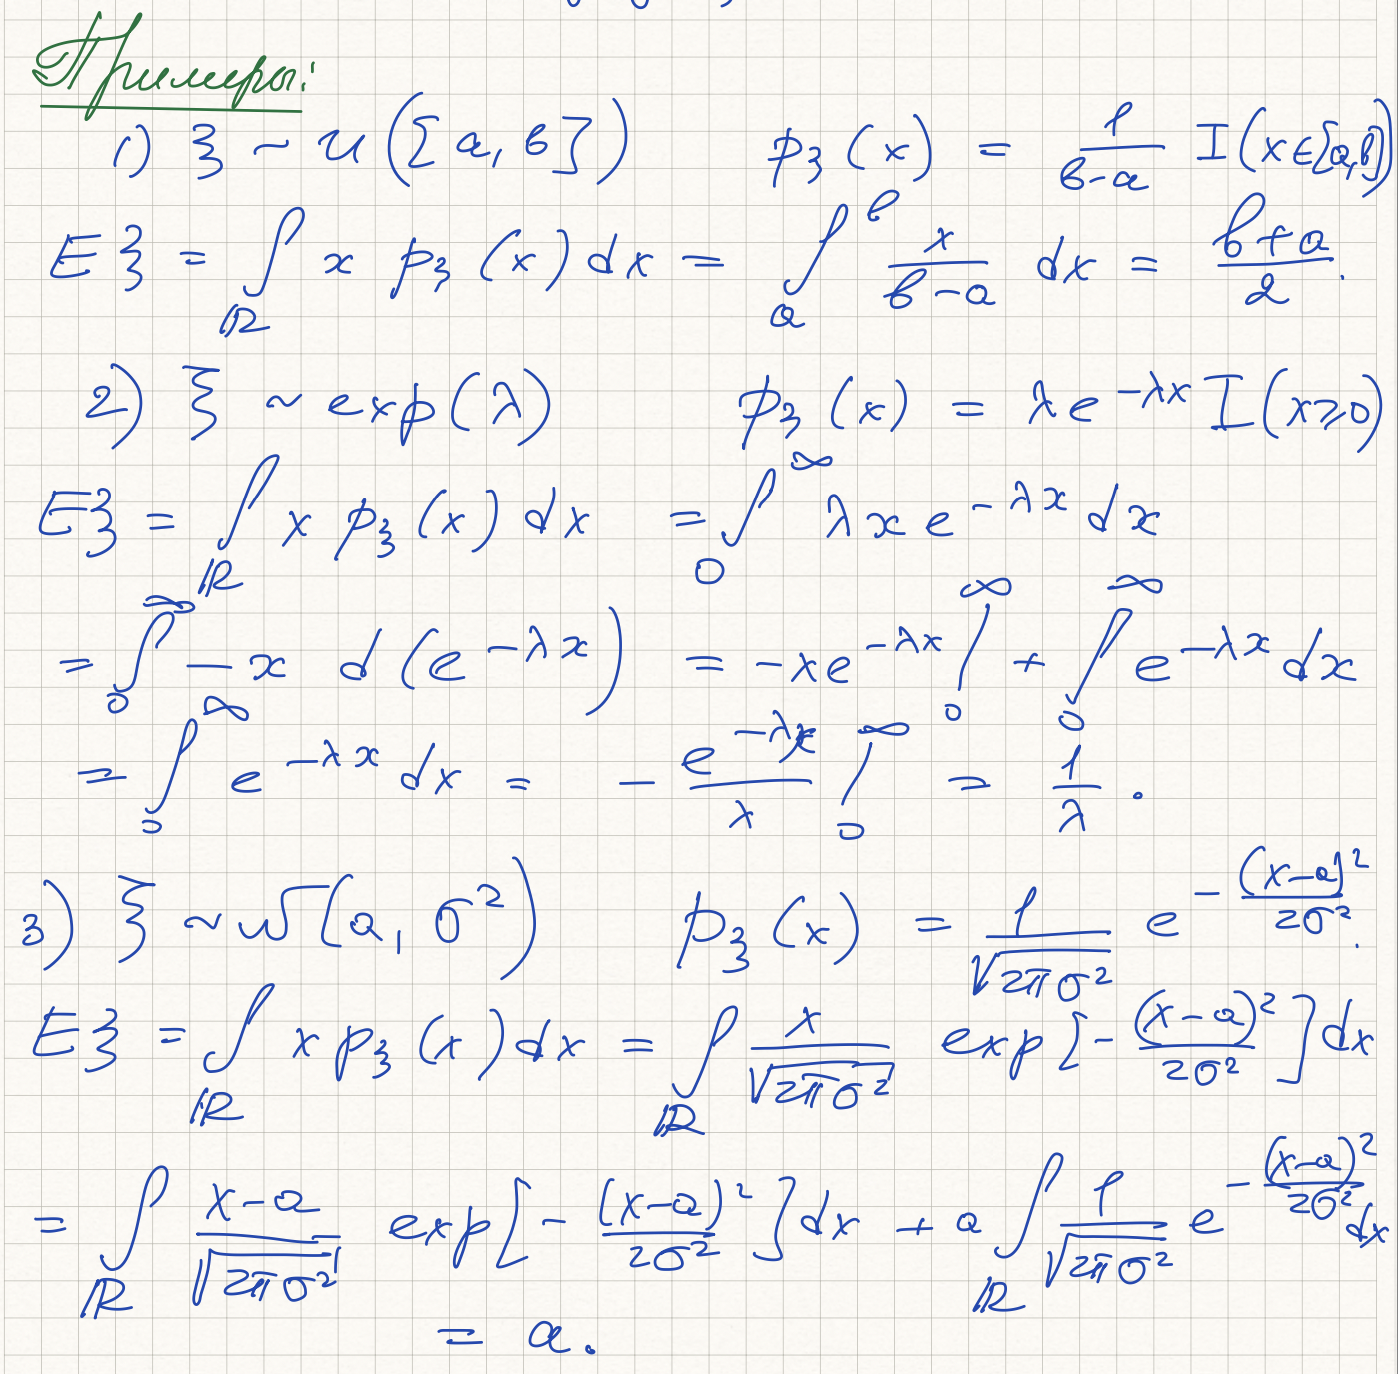
\includegraphics[width=1\linewidth]{sections/sasha/images/expect-examples.png}

\subsubsection*{Свойства мат. ожидания}
\begin{trait}
    \(\forall a \in \R \;:\; \E a\xi = a\cdot\E\xi\)
\end{trait}

\begin{trait}
\label{trait-mathexp-2}
    Если
    \(\xi \geqslant 0\), то \( \E\xi \geqslant 0\)
    
    \hspace{14ex} Если \(\xi \geqslant 0, \E\xi = 0 \), то \( P(\xi = 0) = 1\)
\end{trait}
\begin{proof}
        Так как $\xi \geqslant 0$, то существует последовательность неотриц. простых $\xi_n \uparrow \xi$\\
        Т.к. $\xi_n \leqslant \xi$, то $\E\xi_n \leqslant \E\xi = 0$. Откуда $\E\xi_n = 0$.
        \[\E\xi_n = \sum a_k P(\xi_n \in B_k) = 0.\]
        Значит, $a_k = 0 \implies \xi_n = 0$. Следовательно, $P(\xi = 0) = 1$.
\end{proof}

\begin{trait}
Если $\xi > \eta$ и $\E\xi, \E\eta$ существуют, то $\E\xi \geqslant \E\eta$
\end{trait}
\begin{proof}
    \(\xi - \eta \geqslant 0 \;\Rightarrow \; \E(\xi - \eta) \geqslant 0\), а значит по линейности \( \E\xi  - \E\eta \geqslant 0\)
\end{proof}

\begin{trait}
Если существует $\E\xi$, то $\forall A \in \F$ существует $\E(\xi I_A)$

\hspace{14.8ex}Если $|\E\xi|\, < \infty$, то $\forall A \in \F \; \E(\xi I_A) < \infty$.
\end{trait}
\begin{proof}
    Существует $\E\xi$, то либо $\E\xi^+ < \infty$, либо $\E\xi^- < \infty$
    
    Без ограничения общности пусть $\E\xi^+ < \infty$. Распишем:
    \[\xi I_A = (\xi^+ - \xi^-) I_A = \xi^+ I_A - \xi^- I_A =  (\xi I_A)^+ - (\xi I_A)^-\]
    
    Так как $\xi^+ I_A \leqslant \xi^+$, то $\E\xi^+ I_A \leqslant \infty$. Значит, $\E\xi I_A$ существует.
    
    Доказательство в случае $|\E\xi| < \infty$ аналогично.
\end{proof}

\begin{trait}
Если существует $\E\xi$, то $|\E\xi| \leqslant \E|\xi|$
\end{trait}

\begin{trait}
Если существует $\E\xi$, то \[\forall c \in \R\; \E(c\xi) = c \E\xi\]
\end{trait}

\begin{trait}[Линейность]
Если существует $\E\xi, \E\eta$ существуют и если оба бесконечны, то одинаковых знаков, то 
\[\E(\xi + \eta) = \E\xi + \E\xi\]
\end{trait}

\begin{trait}\label{exp-trait-nine}
Пусть $|\E\xi|, |\E\eta| < \infty$ и $\forall A \in \F$
\[
\E \xi I_A \leqslant \E\eta I_A,
\]
тогда 
\[P(\xi \leqslant \eta) = 1.\]
\end{trait}
\begin{proof}
    Введём \(A = \{\omega: \xi(\omega) > \eta(\omega)\} \in \F\). Перепишем условие:
    \[\E \xi I_A \leqslant \E\eta I_A \implies \E(\eta - \xi) I_A \geqslant 0.\]
    
    Причём $(\eta - \xi) I_A = 0$ при $\xi \leqslant \eta$ и 
    $(\eta - \xi) I_A < 0$ при $\xi > \eta$.
    
    Тогда, $(\eta - \xi) I_A$ неположительная случайная величина и значит мат. ожидание от нее тоже не может быть положительным. С другой стороны выполнено и $\E(\eta - \xi) I_A \geqslant 0$. 
    
    Значит, $\E(\eta - \xi) I_A = 0$ и по свойству~(\ref{trait-mathexp-2}),
    $P((\eta - \xi) I_A = 0) = 1$. Но тогда $P(\xi \leqslant \eta) = 1$.
\end{proof}
\begin{trait}
\label{mathexp-trait-independ}
Если $\xi \indep \eta, \E\xi, \E\eta$~--- существуют и конечны, то $\E(\eta \xi) = \E\eta \cdot \E\xi$
\end{trait}
\begin{proof}
    Прямое следствие теоремы Фубини.
    
    \begin{align*}
        \E(\xi\eta) &= \int_{\Omega} \xi(\omega)\eta(\omega) dP\\
        &= \int_{\R^2}xy dP_{(\xi, \eta)} = \int_{\R^2}xy d(P_\xi \times P_\eta) \\
        &\xlongequal[]{\text{теорема Фубини}} \int_{\R} x dP_\xi \int_{\R} y dP_\eta = \E\eta \E\xi.
    \end{align*}
\end{proof}

\section{Напоминание формулировки теоремы Лебега о мажорируемой сходимости. Теорема о замене переменных в интеграле Лебега. Подсчет математического ожидания от функции от случайной величины. Примеры.}
\begin{theorem}[Лебега о мажорируемой сходимости]
Пусть $\xi_n$~--- случайная величина и
\[|\xi_n| \leqslant \eta,\; \E\eta < \infty\]

\noindentЕсли \(P(\xi_n \to \xi) = P(\{\omega: \xi_n(\omega) \to  \xi(\omega)\}) = 1\), то
\[\E\xi_n \to \E\xi,\; \E|\xi| < \infty,\; \E|\xi_n - \xi| \to 0.\]
\end{theorem}

\begin{theorem}[О замене переменных в интеграле Лебега]
Пусть $X$~--- случайный вектор размерности $k$, $\varphi:\; \R^k \rightarrow \R$~--- бореллевская функция. Тогда если существует $\E\varphi(X)$, то
\[
    \E\varphi(X) = \int_{\R^k}\varphi(x) dP_X
\]
\end{theorem}
\begin{proof}
Рассмотрим случаи
\begin{enumerate}
    \item $\varphi(x) = I(x \in B), B \in \B(\R^k)$.Тогда
    \begin{align*}
        \E\varphi(X) &= \E I(X \in B) = P(X \in B) = P_X(B) = \int_B dP_X\\
        &= \int \varphi(x) dP_X.
    \end{align*}
    \item $\varphi$~--- простая, то верно по линейности интеграла Лебега.
    \item $\varphi \geqslant 0$, то существует возрастающая последовательность простых функций: \\$
    0 \leqslant \varphi_n < \varphi, \varphi_n \uparrow \varphi$.
    \begin{align*}
        \E\varphi(X) = \lim_{n \to \infty}\E\varphi_n(X) = 
         \lim_{n \to \infty}\int\varphi_n(x)dP = \int\varphi(x) dP_X.
    \end{align*}
    \item Для произвольной функции $\varphi = \varphi^+ - \varphi^-$.
\end{enumerate}
\end{proof}

\subsubsection*{Примеры}
\begin{enumerate}
    \item $\xi \sim Bin(n, p)$.\\
    $\xi_1, \ldots, \xi_n \sim Bern(p)$~--- независимые.\\
    $\xi_1 + \ldots + \xi_n \sim Bin(n, p)$. Тогда:\\
    $\E\xi = \E(\xi_1 + \ldots + \xi_n) = \E(\xi_1) + \ldots + \E(\xi_n) = np.$
    \item $\xi \sim \Norm(a, \sigma^2)$.\\
    $\eta \sim \Norm(0, 1) \implies \sqrt{\sigma^2}\eta + a \sim \Norm(a, \sigma^2).$ Это видно из определения нормального распределения.\\
    Так как $\E\eta = 0$, то $\E\xi = \E(\sqrt{\sigma^2}\eta + a) = \sqrt{\sigma^2}\E(\eta) + a = a.$
\end{enumerate}

\section{Дисперсия, ковариация и их свойства. Примеры. Теорема о математическом ожидании произведения независимых случайных величин.}
\begin{definition}[Дисперсия]
\[\D\xi = \E (\xi - \E\xi)^2.\]
\end{definition}

\begin{statement}
\[\D\xi = \E\xi^2 - (\E\xi)^2.\]
\end{statement}
\begin{proof}
Из определения и свойства линейности мат. ожидания.
\end{proof}

\begin{definition}(Ковариация)
\[cov(\xi, \eta) = \E(\xi - \E\xi)(\eta - \E\eta).\]
\end{definition}
\begin{statement}
\[\D\xi = cov(\xi, \xi).\]
\end{statement}

\subsubsection*{Свойства}
\begin{itemize}
    \item $\D\xi \geqslant 0$.
    \item $\D(c\eta) = c^2 \D\eta$.
    \item $cov(\xi, \eta) = \E\xi\eta - \E\xi \cdot \E\eta$.
    \begin{proof}
    Расписать ковариацию и воспользоваться линейностью мат. ожидания.
    \end{proof}
    \item $cov(\xi, \eta) = cov(\eta, \xi).$\\
    $cov(a_1\xi_1 + a_2\xi_2, \eta) = a_1 cov(\xi_1, \eta) + a_2 cov(\xi_2, \eta)$.
    \item $D(\xi_1 + \ldots + \xi_n) = \sum_{i=1}^n\D\xi_i + \sum_{i \neq j} cov(\xi_i, \xi_j).$
    \begin{proof}
    \(\D(\xi_1 + \ldots + \xi_n) = cov(\xi_1 + \ldots + \xi_n, \xi_1 + \ldots + \xi_n) = \sum_{i, j} cov(\xi_i, \xi_j).\)
    \end{proof}
    \item Если $\xi \indep \eta$, то $cov(\xi, \eta) = 0$.
    \item Если $\xi_1, \ldots \xi_n$~--- попарно независимы, то\\
    \(\D(\xi_1 + \ldots + \xi_n) = \D\xi_i + \ldots \D\xi_n\).
\end{itemize}
\begin{definition}(Корреляция)
\[\rho(\xi, \eta) = \frac{cov(\xi, \eta)}{\sqrt{\D\xi}\sqrt{\D\eta}}.\]
\end{definition}

Теорема о мат. ожидании произведения для независимых случайных величин доказана как пункт~(\ref{mathexp-trait-independ}) свойств.

\subsubsection*{Примеры}
\noindent 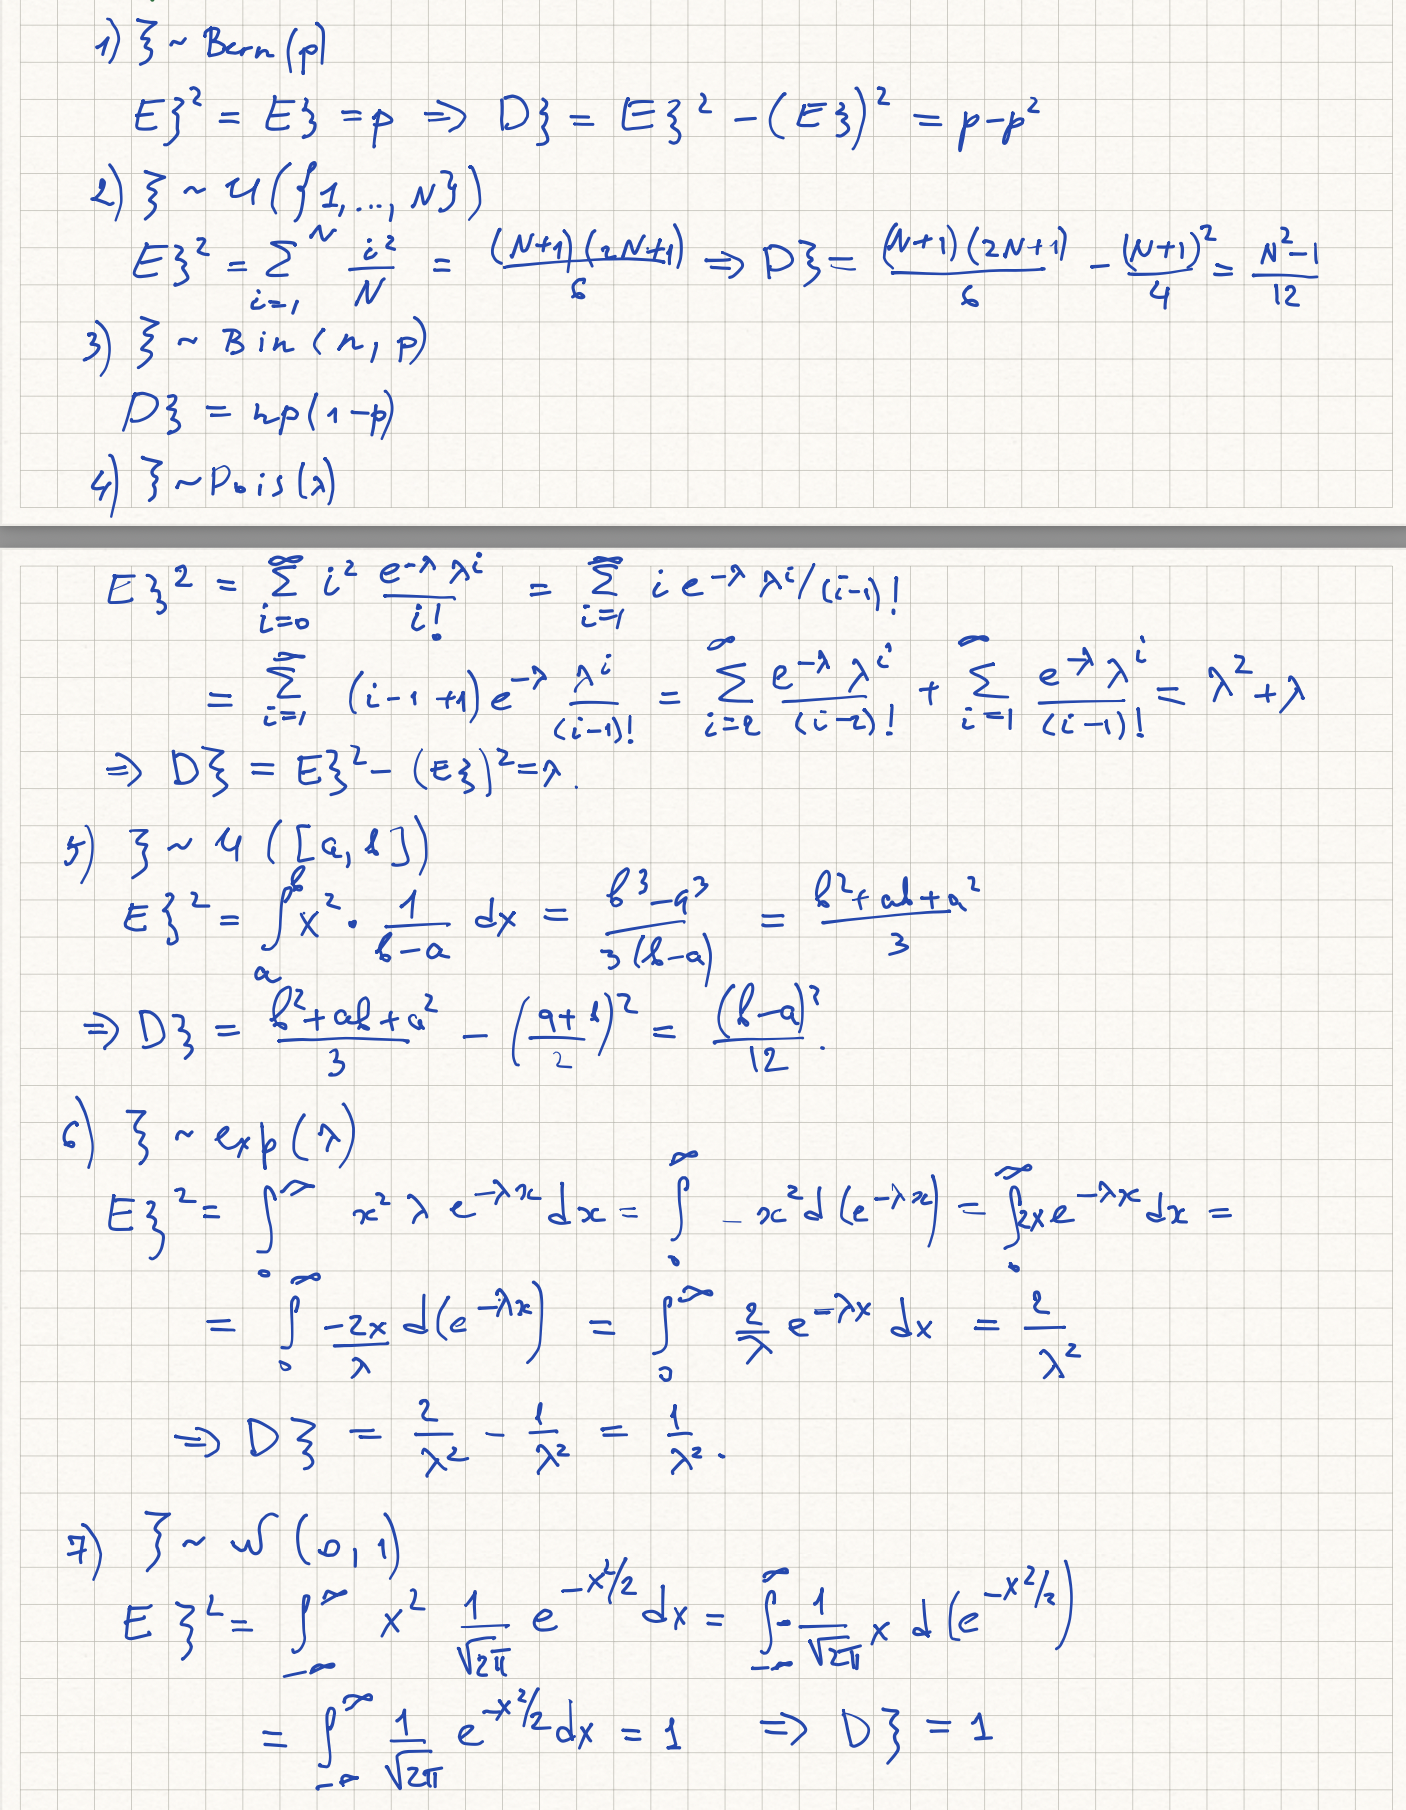
\includegraphics[width=1\linewidth]{sections/sasha/images/expect-example-2.png}
\newpage
\noindent 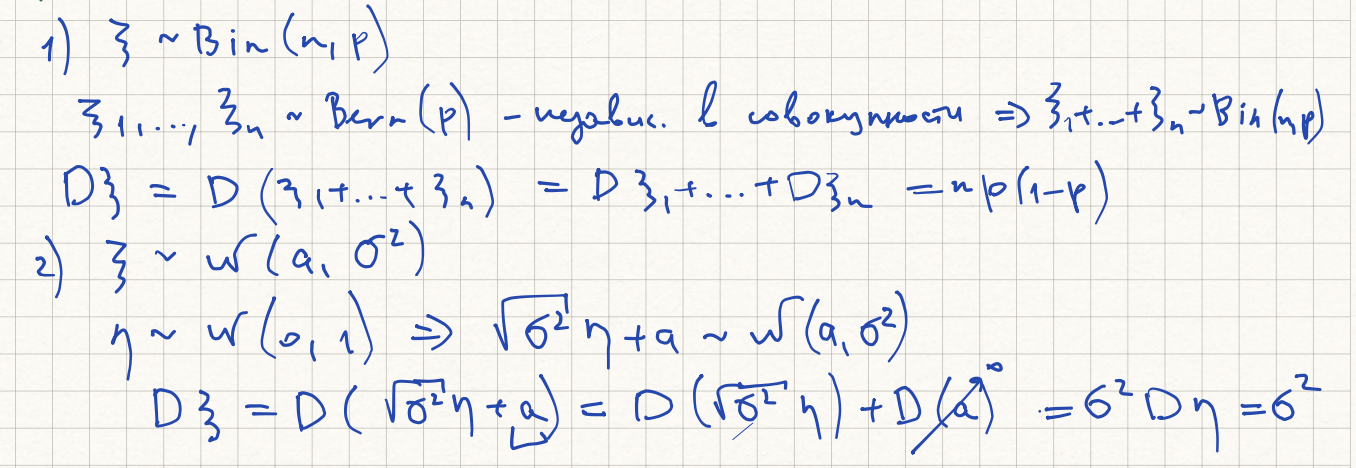
\includegraphics[width=1\linewidth]{sections/sasha/images/expect-disp-ex.png}

\section{Неравенство Коши--Буняковского. Неравенство Маркова. Неравенство Чебышёва. Закон больших чисел в форме Чебышёва. Неравенство Йенсена.}
\begin{theorem}[Неравенство Коши--Буняковского]
Пусть $\E\xi^2 < \infty,\; \E\eta^2 < \infty$.\\
Тогда $\E|\xi\eta| < \infty, \E|\xi\eta| \leqslant \sqrt{\E\xi^2 \E\eta^2}$.
\end{theorem}
\begin{proof}
Пусть $\E\xi^2 = 0$. Тогда $P(\xi = 0) = 1, \E|\xi\eta| = 0$ и неравенство выполнено.

Пусть теперь $\E\xi^2 \neq 0,\; \E\eta^2 \neq 0$. Введем отнормированные величины:
\[\widetilde{\xi} = \frac{\xi}{\sqrt{\E\xi^2}}, \; \widetilde{\eta} = \frac{\eta}{\sqrt{\E\eta^2}}.\]
Тогда для них $\E\widetilde{\xi}^2 = 1,\; \E\widetilde{\eta}^2 = 1$, откуда 
\[\E(|\widetilde{\xi}| - |\widetilde{\eta}|)^2 = 2 - 2\E|\widetilde{\xi} \widetilde{\eta}| \geqslant 0 \implies \E|\widetilde{\xi}\widetilde{\eta}| \leqslant 1.\]

Значит, $\E\frac{|\xi\eta|}{\sqrt{\E\xi^2} \sqrt{\E\eta^2}} \leqslant 1.$
\end{proof}
\begin{corollary}
Корелляция случайных величин лежит в интервале $[-1; 1]$.
\end{corollary}
\begin{corollary}
Равенство в неравенстве Коши--Буняковского достигается тогда и только тогда когда \[\E(|\widetilde{\eta}| - |\widetilde{\xi}|)^2 = 0 \Leftrightarrow P(|\widetilde{\eta}| - |\widetilde{\xi}| = 0) = 1.\]
То есть, когда величины линейно зависимы.
\end{corollary}
\begin{corollary}
Корреляция принимает $\pm 1$ когда случайные величины линейно зависимы.
\end{corollary}

\begin{theorem}[Неравенство Маркова]
Пусть есть неотрицательная случайная величина $\xi$ и $ a\in \R,\; a > 0,\; \E\xi < \infty$.
Тогда 
\[P(\xi \geqslant a) \leqslant \frac{\E\xi}{a}\]
\end{theorem}
\begin{proof}
Верно неравенство $\xi \geqslant a \cdot I(\xi \geqslant a)$, следовательно $\E\xi \geqslant \E a I(\xi \geqslant a) = aP(\xi \geqslant a)$. Для получения искомого неравенства достаточно поделить на $a$.
\end{proof}
\begin{theorem}[Неравенство Чебышёва]
Пусть $\E\xi^2 < \infty,\; \varepsilon > 0$. Тогда
\[P(|\xi - \E\xi| > \varepsilon) \leqslant \frac{\D\xi}{\varepsilon^2}\]
\end{theorem}
\begin{proof}
Сводится к неравенству Маркова введением случайной величины $\eta = (\xi - \E\xi)^2$.
\end{proof}

\begin{theorem}[ЗБЧ в фоме Чебышёва]
Пусть $\xi_1, \ldots \xi_n$~--- независимые в совокупности одинаково распределенные случайные величины. А также существуют $\E\xi_i = a,\; \D\xi_i = \sigma^2$. Тогда 
\[P\left(\left| \frac{\xi_1 + \ldots + \xi_n}{n} - a \right| > \varepsilon\right) \to 0, n\to \infty.\]
\end{theorem}

\begin{theorem}[Обобщение ЗБЧ]
Пусть $\xi_1, \ldots \xi_n:\; \forall i\neq j\; cov(\xi_i, \xi_j) = 0$.\\
А также, дисперсия каждой $\xi_i$ ограничена:
\[\exists C\; \forall i\; \D\xi_i \leqslant C.\]
Если положить $S_n = \xi_1 + \ldots \xi_n,\; \varepsilon > 0$ и взять некую последовательность $w_n \to \infty, n \to \infty$, то верно:
\[
P\left(\frac{|S_n - \E S_n|}{\sqrt{n} \cdot w_n} > \varepsilon\right) \to 0, n \to \infty.
\]
\end{theorem}
\begin{proof}
Пользуемся неравенством Чебышёва: 
\begin{align*}
    P\left(\frac{|S_n - \E S_n|}{\sqrt{n} \cdot w_n} > \varepsilon\right) = P(|S_n - \E S_n| > \varepsilon \sqrt{n} \cdot w_n) \leqslant \frac{\D S_n}{\varepsilon^2 n w_n^2}\\ = \frac{\D \xi_1 + \ldots + \D \xi_n}{\varepsilon^2 n w_n^2} \leqslant \frac{Cn}{\varepsilon^2 n w_n^2} = \frac{C}{\varepsilon^2 w_n^2} \to 0.
\end{align*}
\end{proof}
\begin{lemmanote}
ЗБЧ в фоме Чебышёва из обобщения получается если положить $w_n = \sqrt{n}$.
\end{lemmanote}

\begin{theorem}[Неравенство Йенсена]
Пусть $g:\R \to \R$~--- выпуклая бореллевская функция и $\E|\xi| < \infty$. Тогда $\E g(\xi) \geqslant g(\E\xi)$
\end{theorem}
\begin{proof}
Определение выпуклости:
\[\forall x_o\; \exists \lambda(x_0):\;\; \forall x\;\; g(x) - g(x_0) \geqslant \lambda(x_0)(x-x_0)\]

Положим $x_0 = \E\xi,\; x = \xi$, тогда:
\[g(\xi) - g(\E\xi) \geqslant \lambda(\E\xi)(\xi - \E\xi), \implies\]
\[\E(g(\xi) - g(\E\xi)) \geqslant \lambda(\E\xi)(\E\xi - \E\xi) = 0 \implies  \E g(\xi) - g(\E\xi) \geqslant 0.\]
\end{proof}


\includegraphics[width=1\textwidth]{sections/sasha/images/zbc-iensen-examples.png}

\section{Условное матожидание. Теорема Радона–-Никодима (б/д). Существование и единственность математического ожидания.}
Пусть $\xi$ определена на $\probspace$, $\E|\xi| < \infty$, $\mathcal{G} \subset \F$~--- $\sigma$-алгебра
\begin{definition}
    Условным математическим ожидание $\xi$ при условии $\mathcal{G}$ называется $\mathcal{G}$-измеримая случайная величина $\E(\xi | \mathcal{G})=\eta$, такая что $\forall A \in \mathcal{G} \hookrightarrow \E(\xi I_A)=\E(\eta I_A)$.
\end{definition}

\begin{definition}
    Функция $\nu: \mathcal{G} \rightarrow \R$ называется зарядом, если она счетно-аддитивная.
\end{definition}

\begin{lemmanote}
    Заряд отличается от меры только тем, что может принимать отрицательные значения
\end{lemmanote}

\begin{definition}
    Функция $\nu$ абсолютно непрерывна относительно $P$, если \(\forall A \in \mathcal{G} \hookrightarrow P(A)=0 \Rightarrow \nu(A)=0\).
\end{definition}

\begin{theorem}[Радона--Никодима]\label{radon-nikodim}
    Пусть $\nu$ --- абсолютно непрерывный относительно $P$ заряд. Тогда
    \[ \exists! g: \Omega \rightarrow \R - \mathcal{G} \text{-измеримая, т.ч. } \forall A \in \mathcal{G} \hookrightarrow \nu(A)=\int_A g dP \]
    В данном случае единственность в смысле $P$-почти наверное (какие бы мы не взяли подходящие функции $g$ вероятиность того, что они совпадают, равна 1).
\end{theorem}

\begin{corollary}\label{umo-existence}
    \( \E(\xi|\mathcal{G}) \) существует и единственно $P$-почти наверное
\end{corollary}

\begin{proof}
    \par Рассмотрим $\nu(A)=\E(\xi I_A)$ - заряд. Если $P(A)=0$, то $E\xi I_A=0 \Rightarrow \nu$ - абсолютно непрерывна относительно $P$.
    
    \par Тогда по теореме \nameref{radon-nikodim} \( \exists! g: \Omega \rightarrow \R - \mathcal{G} \text{-измеримая, т.ч. } \forall A \in \mathcal{G} \hookrightarrow \nu(A)=\E \xi I_A = \int_A g dP = EgI_A \). Тогда $g=\E(\xi|\mathcal{G})$ по определению и все доказано.
\end{proof}
\section{Подсчет условного математического ожидания для сигма-алгебры, порожденной разбиением.}
Пусть $\Omega=D_1 \sqcup D_2 \sqcup \ldots$, $P(D_i)>0$, $\mathcal{G}=\sigma(\{D_1, D_2, \ldots\})$

\begin{statement}
    \[ \E(\xi|\mathcal{G})=\sum_i \frac{\E \xi I_{D_i}}{P(D_i)} \cdot I_{D_i} \]
\end{statement}

\begin{proof}
    \( \eta = \sum_i \frac{\E \xi I_{D_i}}{P(D_i)} \cdot I_{D_i} \)
    \begin{enumerate}
        \item $\eta$ - $\mathcal{G}$-измерима, так как $I_{D_i}$ - $\mathcal{G}$-измеримы, а значит их линейная комбинация тоже $\mathcal{G}$-измерима
        
        \item $A \in \mathcal{G} \Rightarrow A = \bigsqcup\limits_{i \in I} D_i$
        
        \[ \E\left(\eta I_A\right)=\E\left(\sum_i \frac{\E \xi I_{D_i}}{P(D_i)} \cdot I_{D_i} \cdot I_A\right)= \]
        
        Заметим, что произведение индикаторов не равно 0, только если $i \in I$.
        
        \[ = \E\left(\sum_{i \in I} \frac{\E \xi I_{D_i}}{P(D_i)} \cdot I_{D_i}\right)=\sum_{i \in I} \frac{\E \xi I_{D_i}}{P(D_i)} \cdot P(D_i)=\sum_{i \in I} \E \xi I_{D_i}=\E\xi I_A \]
    \end{enumerate}
\end{proof}

\section{Свойства условного математического ожидания.}
\begin{enumerate}
    \item \( \E(\xi | \F) = \xi \)
    \begin{proof}
        По определению случайной величины $\xi$ - $\F$-измерима. Также
        \[ \forall A \in \F \hookrightarrow \E(\E(\xi | \F)I_A)=\E(\xi I_A) \]
        Значит, определение выполняется
    \end{proof}
    
    \item Пусть $\mathcal{G}\indep \F_\xi=\{\xi^{-1}(B), B \in \B(\R)\}$ (сигма-алгебра, порожденная $\xi$). Тогда \( \E(\xi | \mathcal{G})=\E \xi \)
    \begin{proof}
        $\E \xi$ является $\G$-измеримым (это константа)
        \[ \forall A \in \G \hookrightarrow \E(\E(\xi|\G)I_A)=\E(\E\xi \cdot I_A)=\E\xi \cdot \E I_A=\E(\xi \cdot I_A) \]
        
        Последний переход сделали в силу независимости $\xi$ и $I_A$. Распишем подробнее: $\xi$ и $I_A$ независимы тогда и только тогда когда для любого $B \in \B(\R)$
        \[ P(\xi \in B, I_A=1)=P(\xi \in B)P(I_A=1)=P(\xi^{-1}(B))P(A) \]
        \[ P(\xi \in B, I_A=0)=P(\xi \in B)P(I_A=0)=P(\xi^{-1}(B))P(\overline{A}) \]
        
        Эти равенства следуют из независимости сигма-алгебр $\G$ и $\F_\xi$
    \end{proof}
    
    \item \( \E(\E(\xi|\G))=\E\xi \)
    \begin{proof}
        Положим в определении матожидания $A=\Omega$. Помним, что $I_\Omega=1$ на всех элементарных исходах. Тогда с одной стороны из определения матожидания
        \[ \E(\E(\xi|\G)\cdot I_\Omega)=\E \xi I_\Omega = \E \xi \]
        
        С другой стороны
        \[ \E(\E(\xi | \G)\cdot I_\Omega)=\E(\E(\xi|\G)) \]
        
        Получаем искомое равенство
    \end{proof}
    
    \item Пусть $\G_1 \subset \G_2 \subset \F$. Тогда 
    \[ \E(\E(\xi|\G_1) | \G_2)=\E(\E(\xi|\G_2)|\G_1)=\E(\xi|\G_1) \]
    \begin{proof}
        По определению \( \E(\xi|\G_1) \) - $\G_1$-измерима $\Rightarrow$ она $\G_2$-измерима (т.к. $\G_1 \subset \G_2$). Тогда по свойству 1
        \[ \E(\E(\xi|\G_1)|\G_2)=\E(\xi|\G_1) \]
        
        Проверим второе равенство: \( \E(\E(\xi|\G_2)|\G_1)=\E(\xi|\G_1) \)
        
        По определению $\E(\xi | \G_1)$ - $\G_1$-измеримо. Значит осталось проверить, что 
        \[ \forall A \in \G_1 \hookrightarrow \E(\E(\xi|\G_1) \cdot I_A)=\E(\E(\xi | \G_2) \cdot I_A) \]
        
        Так как $A \in \G_1$, по определению условного матожидания в $\G_1$ получаем \( \E(\E(\xi | \G_1) \cdot I_A)=\E \xi I_A \)
        
        С другой стороны, $\G_1 \subset \G_2 \Rightarrow A \in \G_2$. Тогда по определению условного матожидания в $\G_2$: \( \E(\E(\xi | \G_2) \cdot I_A)=\E \xi I_A \). Тогда \( \E(\E(\xi | \G_1) \cdot I_A)=\E(\E(\xi | \G_2) \cdot I_A) \) и искомое равенство доказано
    \end{proof}
    
    \item Если $\xi_1 \leqslant \xi_2$ почти наверное, то $\E(\xi_1 | \G) \leqslant \E(\xi_2 | \G)$ почти наверное
    \begin{proof}
        \( \E(\xi_1 | \G), \E(\xi_2 | \G) \) - $\G$-измеримы по определению. Тогда по свойству \ref{exp-trait-nine} матожидания для \( \E(\xi_1 | \G) \leqslant \E(\xi_2 | \G) \) достаточно доказать, что 
        \[ \forall A \in \G \hookrightarrow \E(\E(\xi_1 | \G) I_A) \leqslant \E(\E(\xi_2 | \G) I_A) \]
        
        Пусть $A \in \G$. Тогда по определению условного матожидания
        \[ \E(\E(\xi_1 | \G) I_A)=\E(\xi_1 I_A) \leqslant \E(\xi_2 I_A) = \E(\E(\xi_2 | \G)I_A) \]
    \end{proof}
    
    \item \( \E(c_1 \xi_1 + c_2 \xi_2 | \G)=c_1 \E(\xi_1|\G)+c_2 \E(\xi_2 | \G) \)
    \begin{proof}
        \( c_1 \E(\xi_1|\G)+c_2 \E(\xi_2 | \G) \) - $\G$-измеримо. Если $A \in \G$ выполнено (применяем линейность матожидания и определение условного матожидания)
        
        \[ \E([c_1 \E(\xi_1 | \G) + c_2 \E(\xi_2|\G)]I_A)=c_1 \E[\E(\xi_1|\G) I_A]+c_2 \E[\E(\xi_2 | \G) I_A]= \]
        \[ = c_1 \E\xi_1 I_A +c_2 \E \xi_2 I_A = \E[(c_1 \xi_1 + c_2 \xi_2) I_A] \]
    \end{proof}
    
    \item \( \E(|\xi| \: | \: \G) \geqslant |\E(\xi|\G)| \) почти наверное
    \begin{proof}
        \( -|\xi| \leqslant \xi \leqslant |\xi| \). Тогда по свойству 5 получаем \( E(-|\xi| \: | \: \G) \leqslant \E(\xi | \G) \leqslant \E(|\xi| \: | \: \G) \). Отсюда по свойству 6: \( -E(|\xi| \: | \: \G) \leqslant \E(\xi | \G) \leqslant \E(|\xi| \: | \: \G) \Rightarrow \E(|\xi| \: | \: \G) \geqslant |\E(\xi|\G)| \)
    \end{proof}
    
    \item \( P(\xi_n \rightarrow \xi)=1, \: |\xi_n|\leqslant \eta, \: \E \eta < \infty \Rightarrow P(\E(\xi_n|\G) \rightarrow \E(\xi | \G))=1 \) (оставим без доказательства, оно аналогично теореме Лебега)\label{umo-lim-trait}
    
    \item Если $\eta$ - $\G$-измерима, то $\E(\xi \eta | \G)=\eta \E(\xi|\G)$
    \begin{proof}
        \( \eta \E(\xi | \G) \) - $\G$-измерима. Будем доказывать сначала для простых $\eta$, потом усложнять
        \begin{itemize}
            \item \( \eta=I_A, \: A \in \G \). Пусть \( \widetilde{A} \in \G \). Тогда
            \[ \E(\eta \E(\xi | \G) I_{\widetilde{A}})=E(I_A \E(\xi | \G) I_{\widetilde{A}})=\E(\E(\xi | \G) I_{A \cap \widetilde{A}})\stackrel{1}{=}\E(\xi I_{A \cap \widetilde{A}})=\E(\xi I_A I_{\widetilde{A}})=\E(\xi \eta I_{\widetilde{A}}) \]
            
            Переход 1 выполнен по определению условного матожидания для $\xi$.
            
            \item \( \eta = \sum_{i=1}^n c_i I_{A_i}, \: A_i \in \G, \: c_i \in \R \)
            
            \[ \E(\eta \E(\xi | \G) I_{\widetilde{A}})=\sum_{i=1}^n c_i \E(I_{A_i} \E(\xi | \G) I_{\widetilde{A}})\stackrel{2}{=}\sum_{i=1}^n c_i \E(\xi I_{A_i} I_{\widetilde{A}})=\E(\xi \eta I_{\widetilde{A}}) \]
            
            Переход 2 выполнен в силу первого пункта доказательства
            
            \item $\eta$ - произвольная. Тогда существует последовательность простых случайных величин $\eta_n \rightarrow \eta$, $|\eta_n|\leqslant |\eta|$. По свойству 8 выполнено \( \E(\xi \eta|\G) \stackrel{\text{п.н.}}{\rightarrow} \E(\xi \eta | \G) \), так как $\xi \eta_n \rightarrow \xi \eta, \: |\xi \eta_n| \leqslant |\xi \eta|, \E|\xi \eta| < \infty$ (последнее из требований в определении УМО). Из второго пункта доказательства получаем
            \[ \E(\xi \eta_n | \G)=\eta_n \E(\xi | \G) \]
            
            Переходя к пределу по $n$ получим \( \E(\xi \eta | \G)=\eta \E(\xi | \G) \)
        \end{itemize}
    \end{proof}
\end{enumerate}

\section{Условное распределение и условная плотность. Критерий существования условной плостности.}
\begin{definition}
    \( \E(\xi | \eta=y)=\varphi(y) \) (равенство в смысле $P_\eta$-почти наверное), $\varphi: \R^n \rightarrow \R$ - борелевская, такая что 
    \[ \forall B \in \B(\R^n) \hookrightarrow \E \xi I(\eta \in B)=\int_B \varphi dP_\eta \]
\end{definition}

\begin{lemmanote}
    \( \E(\xi | \eta = y)=\varphi(y) \Leftrightarrow \E(\xi | \eta)=\varphi(\eta) \)
\end{lemmanote}

\begin{proof}
    \begin{itemize}
        \item[$\Rightarrow$:] Пусть $\varphi(y)=\E(\xi | \eta = y)$. Очевидно, что $\varphi(\eta)$ - $\F_\eta$-измерима (если берем борелевскую функцию от измеримой случайной величины измеримость сохраняется). Нужно проверить, что 
        
        \[ \forall A \in \F_\eta \hookrightarrow \E \xi I_A = \E \varphi(\eta) I_A \]
    
        Так как $A \in \F_\eta$, то $\exists B \in \B(\R^n): \: A=\eta^{-1}(B)$ Тогда, используя определение $\E(\xi | \eta = y)$, получаем
         \[ \E \xi I_A = \E \xi I(\eta \in B)=\int_B \varphi dP_\eta = \int_{\R^n} \varphi I_B dP_\eta \stackrel{1}{=} \int_\Omega \varphi(\eta) I_A dP = \E \varphi(\eta) I_A \]
    
        Переход 1 делаем при помощи теоремы о замене переменных в интеграле Лебега.
        
        \item[$\Leftarrow$:] Пусть $\E(\xi|\eta)=\varphi(\eta)$. Тогда $\varphi(\eta)$ - $\F_\eta$-измерима (по определению УМО). Тогда для произвольного $B \in \B(\R)$ выполнено $[\varphi(\eta)]^{-1}(B) \in \F_\eta$. Следовательно, по определению $\F_\eta$ 
        
        \[ \exists A \in \B(\R^n): [\varphi(\eta)]^{-1}(B)=\eta^{-1}(A) \]
        
        Применяя $\eta$ к обеим частям равенства получим (???), что $A = \varphi^{-1}(B)$, а значит $\varphi$ - борелевская (прообраз произвольного борелевского множества оказался борелевским)
        
        Осталось показать, что \( \forall B \in \B(\R^n) \hookrightarrow \E \xi I(\eta \in B)=\int_B \varphi dP_\eta \)
        
        \( \E \xi I(\eta \in B)=\E \xi I_A \), где \( A = \eta^{-1}(B) \in \F_\eta \). Тогда
        
        \[ \E \xi I(\eta \in B)=\E \xi I_A\stackrel{2}{=}\E\E(\xi | \eta) \cdot I_A\stackrel{3}{=} \E\varphi(\eta) I_A = \int_\Omega \varphi(\eta) I_A dP \stackrel{4}{=} \int_\R \varphi I_B dP_\eta = \int_B \varphi dP_\eta \]
        
        Переход 2 сделали по определению УМО, 3 - по условию леммы, 4 - по теореме о замене переменных.
    \end{itemize} 
\end{proof}

\begin{definition}
    Условное распределение $\xi$ (в общем случае это может быть вектор) при условии $\eta=y$ есть 
    \[ P_{\xi|\eta}(B) := \E(I(\xi \in B)|\eta) \]
    \[ P_{\xi|\eta = y}(B) = P(\xi \in B|\eta = y) := \E(I(\xi \in B)|\eta = y) \]
\end{definition} 

\begin{definition}
    Функция $f(x, y) = p_{\xi|\eta = y}(x)$ ($x \in \R^k, y \in \R^n$) - условная плотность, если 

    \[ \forall y \in \R^n, \forall B \in \mathcal{B}(\R^k) \ P_{\xi|\eta = y}(B) = \int\limits_{B}p_{\xi|\eta = y}(x)dx \]
\end{definition}

\begin{statement}[критерий существования условной плотности]
    Пусть $p_{\xi, \eta}$ - плотность абсолютно непрерывного случайного вектора $(\xi, \eta)$, $p_\eta$ - плотность $\eta$, тогда
    
    \[ p_{\xi|\eta = y}(x) = \begin{cases} 
    \frac{p_{\xi, \eta}(x, y)}{p_\eta(y)}, & p_\eta(y) \ne 0 \\ 
    0, & \text{иначе}
    \end{cases} \]
\end{statement} 

\begin{proof}
    Надо проверить выполнение определения условной плотности. $y \in \R^n, B \in \mathcal{B}(\R^k)$.\\ Должно выполняться $P_{\xi|\eta = y}(B) = \E(I(\xi \in B)|\eta = y) = \int\limits_{B}p_{\xi|\eta = y}(x)dx = f(y)$. То есть доказываем равенство УМО какому-то выражению, то есть надо доказать, что выражение удовлетворяет определению УМО, а именно  
    \begin{enumerate}
        \item $f(y)$ борелевская
        
        $\int\limits_{B}p_{\xi|\eta = y}(x)dx = 0$, если $p_\eta(y) = 0$. Пусть $p_\eta(y) \ne 0$. Тогда 
        \[ \int\limits_{B}p_{\xi|\eta = y}(x)dx = \int\limits_{B} \frac{p_{\xi, \eta}(x, y)}{p_\eta(y)} dx = \frac{1}{p_\eta(y)} \int\limits_{B} p_{\xi, \eta}(x, y) dx \] 
        Произведение двух борелевских функций (плотность есть борелевская функция) тоже борелевская функция 
        
        \item $\forall A \in \mathcal{B}(\R^n) \ \  \E I(\xi \in B) I(\eta \in A) = \int\limits_A f\ dP_\eta$ (по определению $\E(\xi|\eta=y)$: вместо случайной величины $\xi$ в определении выступает $I(\xi \in B)$).
        
        Возьмем $A \in \mathcal{B}(\R^n)$ \\
        $\E I(\xi \in B, \eta \in A) = P(\xi \in B, \eta \in A) = \int\limits_{A \times B} p_{\xi, \eta}(x, y) \ dx\ dy = \int\limits_{A} \Big ( \int\limits_{B}p_{\xi, \eta}(x, y) \ dx \Big ) dy =$ \\ $ =(\Sigma = \{ y, p_\eta(y) = 0 \} )= \int\limits_{A \setminus \Sigma} \Big ( \int\limits_{B}p_{\xi, \eta}(x, y) \ dx \Big ) dy \stackrel{1}{=} 
        \int\limits_{A \setminus \Sigma} \Big ( \int\limits_{B}p_{\xi| \eta = y}(x) \cdot p_{\eta}(y) \ dx \Big ) dy  =$ \\ $= \int\limits_{A \setminus \Sigma} \Big ( \int\limits_{B}p_{\xi| \eta = y}(x)\ dx \Big ) \cdot p_{\eta}(y) \ dy = \int\limits_{A \setminus \Sigma} \Big ( \int\limits_{B}p_{\xi| \eta = y}(x)\ dx \Big ) \cdot \ dP_\eta \stackrel{2}{=} \int\limits_{A} \Big ( \int\limits_{B}p_{\xi| \eta = y}(x)\ dx \Big ) \cdot \ dP_\eta = \int\limits_{A} f \ dP_\eta $
        
        Переход 1 сделали по определению функции $p_{\xi, \eta}$ из условия теоремы, а в переходе 2 вернули $\Sigma$, так как интеграл по нему равен 0.
    \end{enumerate}
\end{proof} 

\section{Подсчет условного математического ожидания с помощью условной плотности.}
\begin{statement}[подсчет условного матожидания]
    Пусть $\varphi: \R^k \rightarrow \R$ --- борелевская, $p_{\xi|\eta=y}(x)$ --- условная плотность $P_{\xi|\eta=y}$. Тогда 
    \[ \E(\varphi(\xi)|\eta=y)=\int_{\R^k} \varphi(x) p_{\xi|\eta=y}(x)dx \]
\end{statement}

\begin{proof}
    Тут мы будем доказывать не как обычно через определение УМО, а докажем равенство напрямую:
    \begin{enumerate}
        \item Пусть $\varphi = I_B, B \in \mathcal{B}(\R^k)$, тогда
        $$\int\limits_{\R^k} \varphi(x) p_{\xi|\eta = y}(x) dx = \int\limits_{\R^k} I_B p_{\xi|\eta = y}(x) dx = \int\limits_B p_{\xi|\eta = y}(x) dx = P(\xi \in B | \eta = y) = \E(\varphi(\xi)| \eta = y)$$
        
        \item В силу линейности УМО и интеграла Лебега, для простых $\varphi(x)=\sum_{i=1}^n c_i I_{A_i}$ получаем
        $$\int_{\R^k} \varphi(x) p_{\xi|\eta=y}(x) dx=\sum_{i=1}^n c_i \int_{A_i} p_{\xi|\eta=y}(x) dx=$$
        $$=\sum_{i=1}^n c_i \E (I(\xi \in A_i) | \eta=y)=\E \left(\sum_{i=1}^n c_i I(\xi \in A_i) | \eta = y\right)=\E(\varphi(\xi)|\eta=y)$$
        
        \item Пусть $\E|\varphi(\xi)| < \infty$. Тогда $\exists \varphi_n \rightarrow \varphi: \: \varphi_n$ - простая, $|\varphi_n| \leqslant |\varphi|$. Мы знаем из прошлого пункта, что
        \[ \int_{\R^k} \varphi_n(x) p_{\xi | \eta=y}(x)dx=\E(\varphi_n(\xi) | \eta=y) \]
        
        Хотим перейти к пределу. Если бы слева был интеграл по обычному распределению, то могли бы спокойно применить теорему Лебега о мажорируемой сходимости и получить что нужно, так как мы знаем, что матожидание $\varphi_n$ существует. Но по следствию \ref{umo-existence} из теоремы \nameref{radon-nikodim}, получаем, что условное матожидание для $\varphi_n$ тоже существует, а значит тоже можем применить теорему Лебега. Справа делаем предельный переход по свойству \ref{umo-lim-trait} условного матожидания. Получаем, что
        \[ \E(\varphi(\xi) | \eta=y)=\int_{\R^k} \varphi(x) p_{\xi| \eta=y}(x) dx \]
\end{enumerate}
\end{proof}

\begin{lemmanote}
    В предельном переходе, справа будет сходимость почти наверное, но этого нам достаточно для условного матожидания
\end{lemmanote}
\section{Простейшее симметричное случайное блуждание. Траектории простейшего симметричного случайного блуждания. Принцип отражения.}
Пусть $\xi_1, \xi_2...$ - НОР $P(\xi_1 = 1) = P(\xi_1 = -1) = \frac{1}{2}$
\begin{definition}
$S_0 = 0, ..., S_n = \xi_1 + .. + \xi_n$ - простейшее симметричное случайное блуждание
\end{definition}
\begin{definition} Зафиксируем $\omega \in \Omega$, то
$\{S_n(\omega), n \in \Z_{+}\}$ - траектория
\end{definition}
$P(S_n = k) = (\frac{1}{2})^n C_n^x$,\;\; где $x - (n-x) = k \;\Rightarrow\; x = \frac{n+k}{2} \;\Rightarrow\; P(S_n = k) =(\frac{1}{2})^n C_n^{\frac{n+k}{2}}$
\\
\\
\textbf{Задача:}  Пусть k > 0. $P(S_1 > 0, S_2 > 0,..., S_n = k) = ?$
Для начала заметим, что первым шагом мы в любом случае должны пойти наверх, то есть начальная точка 1 а не 0. Найдем обратную величину: кол-во траекторий, пересекающих ноль. Между каждой такой траекторией и траекторией из 1 в $-k$ можно задать биективное отображение (просто отражаем относительно первой точки пересечения с нулем).\\ Посчитаем количество траекторий, которые ведут в $(n, -k), S_1 > 0$ = количество тракторий в  $(n, k)$, пересекающих 0, $ S_1 > 0$ =  количество траекторий из (1, 1) в  $(n, -k)$ =  $C_{n-1}^{\frac{n-k - 2}{2}}$, откуда  $P(S_1 > 0, S_2 > 0,..., S_n = k) = (\frac{1}{2})^n (C_{n-1}^{\frac{n+k-2}{2}} - C_{n-1}^{\frac{n-k-2}{2}}) = (\frac{1}{2})^n (C_{n-1}^{\frac{n+k}{2}} - C_{n-1}^{\frac{n-k}{2}})$
\section{Закон повторного логарифма для простейшего симметричного случайного блуждания (б/д). Лемма Бореля–-Кантелли и ее применение.}
\begin{theorem} Для простейшего симметричного блуждания верно, что
$
P\brackets{\overline{\lim\limits_{n \to \infty}}\frac{|S_n|}{\sqrt{2n\cdot lnlnn}} = 1} = 1
$\\
\end{theorem}
\vspace{-4ex}
\begin{figure}[h] \begin{minipage}[h]{0.5\linewidth}
    \center{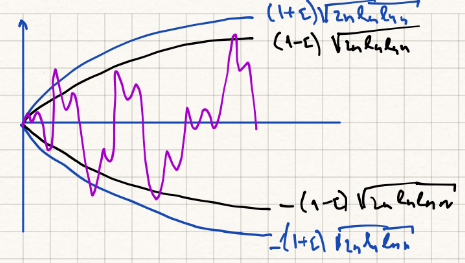
\includegraphics[width=1\textwidth]{images/tv4.png}}
\end{minipage}
\begin{minipage}[h]{0.5\linewidth}
    То есть для почти всех траекторий $S_n$ конечное количество раз больше единицы и бесконечное количество раз меньше единицы. На рисунке это значит, что траекторий пересекает синюю кривую конечное число раз, а черную бесконечное число раз.
\end{minipage}
\end{figure}
% 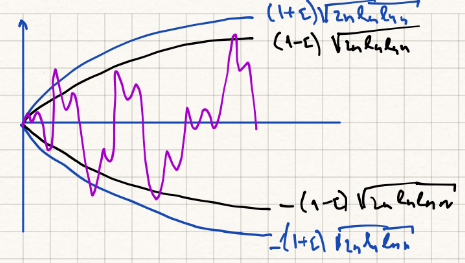
\includegraphics[width=0.3\textwidth]{images/tv4.png}
% То есть для почти всех траекторий $S_n$ конечное количество раз больше единицы и бесконечное количество раз меньше единицы. На рисунке это значит, что траекторий пересекает синюю кривую конечное число раз, а черную бесконечное число раз.
\begin{definition} Пусть $A_1\ A_2, \ldots \in \F$, тогда событие $A_n \text{ б.ч.} = \bigcap\limits_{n = 1}^\infty\bigcup\limits_{k \geqslant n}^\infty A_k$ (бесконечно часто), то есть множество тех элементарных исходов, которые попадают в бесконечное множество событий.
\end{definition} 
\begin{theorem}\textbf{Лемма Бореля-Кантелли}
\begin{enumerate}
    \item Если $\sum\limits_{n = 1}^\infty P(A_n) < \infty$, то $P(A_n \text{ б.ч.}) = 0$
    \item Если $A_1, A_2, \ldots$ независимы и $\sum\limits_{n = 1}^\infty P(A_n) = \infty$, то $P(A_n \text{б.ч.}) = 1$
\end{enumerate}
\end{theorem}

\begin{proof}
   1. $
    P(A_n \text{ б.ч.}) = P\brackets{\bigcap\limits_{n \in \N}\bigcup\limits_{m \geqslant n}A_m} = \lim\limits_{n \to \infty} P\brackets{\bigcup\limits_{m \geqslant n}A_m} \leqslant \lim\limits_{n \to \infty} \sum\limits_{m \geqslant n} P(A_m) = 0
    $\\
    Где второе равенство по теореме о непрерывности меры \\
    2.
    $
         P(A_n \text{ б.ч.}) = P\brackets{\bigcap\limits_{n \in \N}\bigcup\limits_{m \geqslant n}A_m} =  1 - P\brackets{\bigcup\limits_{n \in \N}\bigcap\limits_{m \geqslant n}\overline{A_m}} = 1 - \lim\limits_{n \to \infty} P\brackets{\bigcap\limits_{m \geqslant n} \overline{A_m}} = 1 - \lim\limits_{n \to \infty} \prod\limits_{m \geqslant n} P\brackets{\overline{A_m}} =$ \\
         $= 1 - \lim\limits_{n \to \infty} \exp\brackets{\sum\limits_{m \geqslant n} ln\brackets{1 - P(A_m)}} \geqslant 1 - \lim\limits_{n \to \infty} \exp\brackets{-\sum\limits_{m \geqslant n} P(A_m)} = 1
   $\\
    Где неравенство за счет ряда Тейлора для логарифма.
\end{proof}
\textbf{Пример применения леммы Бореля–Кантелли}

Пусть $\xi_1, \xi_2, \ldots \sim Exp(1)$ и независимы. Доказать, что $P\brackets{\overline{\lim\limits_{n \to\infty}} \frac{\xi_n}{ln \: n} = 1} = 1$
\begin{enumerate}
    \item Докажем, что $P\brackets{\overline{\lim\limits_{n \to\infty}} \frac{\xi_n}{ln \: n} \geqslant 1} = 1$
    \begin{multline*}
        P\brackets{\overline{\lim\limits_{n \to\infty}} \frac{\xi_n}{ln \: n} \geqslant 1} = 1 \Longleftrightarrow P\brackets{\forall \eps > 0 \ \  \forall k \ \exists n \geqslant k: \: \frac{\xi_n}{ln \: n} \geqslant 1 - \eps} = 1 \Longleftrightarrow \\
        \Longleftrightarrow P\brackets{\forall m \in \N \ \ \forall k \ \exists n \geqslant k: \: \frac{\xi_n}{ln \: n} \geqslant 1 - \frac{1}{m}} = 1 \Longleftrightarrow P\brackets{\bigcap\limits_{m = 1}^\infty \bigcap\limits_{k = 1}^\infty \bigcup\limits_{n = k}^\infty \: \frac{\xi_n}{ln \: n} \geqslant 1 - \frac{1}{m}} = 1 \Longleftrightarrow \\
        \Longleftrightarrow \lim\limits_{m \to \infty} P\brackets{\brackets{\frac{\xi_n}{ln \: n} \geqslant 1 - \frac{1}{m}} \text{ б.ч.}} = 1
    \end{multline*}
    $
    \sum\limits_{n = 1}^\infty P\brackets{\frac{\xi_n}{ln \: n} \geqslant 1 - \frac{1}{m}} = \sum\limits_{n = 1}^\infty P\brackets{\xi_n \geqslant \brackets{1 - \frac{1}{m}}ln \: n} = \sum\limits_{n = 1}^\infty \Big (
    \int\limits_{ln \ n (1 - \frac{1}{m})}^{+\infty} e^{-x} dx \Big ) = $\\ $ \sum\limits_{n = 1}^\infty \brackets{e^{-\brackets{1 - \frac{1}{m}}ln\:n}} = \sum\limits_{n = 1}^\infty \brackets{n^{-1 + \frac{1}{m}}} = \infty
    $
    
    Тогда по лемме Бореля-Кантелли событие происходит бесконечно часто, а значит первая часть утверждения доказана.
    
    \item Докажем, что $P\brackets{\overline{\lim\limits_{n \to\infty}} \frac{\xi_n}{ln \: n} \leqslant 1} = 1$
    \begin{multline*}
        P\brackets{\overline{\lim\limits_{n \to\infty}} \frac{\xi_n}{ln \: n} \leqslant 1} = 1 \Longleftrightarrow P\brackets{\forall \eps > 0 \ \ \exists k \ \forall n \geqslant k: \: \frac{\xi_n}{ln \: n} \leqslant 1 + \eps} = 1 \Longleftrightarrow \\
        \Longleftrightarrow P\brackets{\overline{\exists m \in \N \ \  \forall k \ \exists n \geqslant k: \: \frac{\xi_n}{ln \: n} > 1 + \frac{1}{m}}} = 1 \Longleftrightarrow P\brackets{\bigcup\limits_{m = 1}^\infty \bigcap\limits_{k = 1}^\infty \bigcup\limits_{n = k}^\infty \: \frac{\xi_n}{ln \: n} > 1 + \frac{1}{m}} = 0 \Longleftrightarrow \\
        \Longleftrightarrow \lim\limits_{m \to \infty} P\brackets{\brackets{\frac{\xi_n}{ln \: n} > 1 + \frac{1}{m}} \text{ б.ч.}} = 0
    \end{multline*}
    $
    \sum\limits_{n = 1}^\infty P\brackets{\frac{\xi_n}{ln \: n} > 1 + \frac{1}{m}} = \sum\limits_{n = 1}^\infty P\brackets{\xi_n > \brackets{1 + \frac{1}{m}}ln \: n} = \sum\limits_{n = 1}^\infty \Big (
    \int\limits_{ln \ n (1 + \frac{1}{m})}^{+\infty} e^{-x} dx \Big ) =$ \\ $= \sum\limits_{n = 1}^\infty \brackets{e^{-\brackets{1 + \frac{1}{m}}ln\:n}} = \sum\limits_{n = 1}^\infty \brackets{n^{-1 - \frac{1}{m}}} < \infty
    $
    
    Тогда по лемме Бореля-Кантелли вероятность отрицания события равна нулю, а значит вероятность самого события единица, то есть вторая часть (как и все утверждение) доказаны.
\end{enumerate}
\section{Теорема Муавра–-Лапласа (локальная и интегральная, первая с доказательством) и теорема Пуассона.}
\begin{theorem}[Локальная теорема Муавра-Лапласа]
Пусть \( \nu_n \sim Bin(n, p)\) и есть \(\varphi(n) = \overline{\overline{o}}(n^{2/3})\), то верно:

\[\sup_{k\in Z_+:\;\; |k-np|\leqslant \varphi(n)}\left| \frac{\mathbb{P}(\nu_n=k)}{\frac{1}{\sqrt{np(1-p)}} \psi\left(\frac{k-np}{\sqrt{np(1-p)}}\right) } - 1 \right| \xrightarrow[n\to \infty]{} 0 \;\;\;
\text{, где }
\psi(x)=\frac{1}{\sqrt{2 \pi}}e^{-\frac{x^2}{2}}.\]
\end{theorem}
\begin{proof}
Нам потребуется формула Стирлинга: \(\mathlarger{n! \sim \sqrt{2 \pi n} \left( \frac{n}{e} \right)^n}\) при \(n\! \rightarrow\! \infty\). Теперь распишем рассматриваемую вероятность:
\[\mathbb{P}(\nu_n = k) = C_n^k p^k (1-p)^{n-k} = \frac{n!}{k!(n-k)!} p^k (1-p)^{n-k} \sim \frac{\sqrt{2 \pi n} \left( \frac{n}{e} \right)^n}{2 \pi \sqrt{k(n-k)}\left( \frac{k}{e}\right)^k \left( \frac{n-k}{e} \right)^{n-k}}p^k (1-p)^{n-k} =\]
\[= \frac{1}{\sqrt{2 \pi n}} \frac{1}{\sqrt{\frac{k}{n}(1 - \frac{k}{n})}} \left( \frac{np}{k} \right)^k \left( \frac{n (1-p)}{n-k} \right)^{n-k} = \frac{1}{\sqrt{2 \pi n p(1-p)}} \exp \left[-n \cdot g \left( \frac{k}{n} \right) \right],\]
где \(\mathlarger{g(x) = x \ln \left( \frac{x}{p} \right) + (1-x) \ln \left( \frac{1-x}{1-p} \right)}\). Займёмся её исследованием:
\[g'(x) = \ln \left( \frac{x}{p} \right) - \ln \left( \frac{1-x}{1-p} \right) \;\;\;\; g''(x) = \frac{1}{x} + \frac{1}{1-x}\]
\[g(p) = 0, \; g'(p)=0,\; g''(p)=\frac{1}{p(1-p)}\]
\[\text{Приблизим по Тейлору в окрестности p:} \;\;\;\; g(x) = \frac{1}{2}\frac{(x-p)^2}{p(1-p)} + \underline{\underline{O}}((x-p)^3)\]
Подставим это приближение в исходное выражение:
\[\mathbb{P} (\nu_n = k) = \frac{\exp \left[ -n \cdot \left( \frac{1}{2p(1-p)} \left( \frac{k}{n} - p \right)^2 + \underline{\underline{O}}\left( (\frac{k}{n} - p)^3 \right) \right)\right]}{\sqrt{2 \pi n p (1-p)}} = \frac{\exp \left[ -\frac{(k-np)^2}{2np(1-p)} + \underline{\underline{O}} \left( \frac{(k - np)^3}{n^2} \right) \right]}{\sqrt{2 \pi n p (1-p)}}\]
Учитывая \(\mathlarger{|np-k| \leqslant \varphi(n) = \overline{\overline{o}}(n^{\frac{2}{3}})}\), получим \(\mathlarger{ \mathbb{P}(\nu_n = k) = \frac{\exp \left[ -\frac{(k-np)^2}{2np(1-p)}(1 + \overline{\overline{o}}(1)) \right]}{\sqrt{2 \pi n p (1-p)}} } \) при \( n \rightarrow \infty \).
\end{proof}

\begin{theorem}[Интегральная теорема Муавра-Лапласа]
Пусть \( \nu_n \sim Bin(n, p)\) и есть \(\varphi(n) = \overline{\overline{o}}(n^{2/3})\). Тогда равномерно по всем $k \in \R:\;|k - np| < \varphi(n)$:

\[P(\nu_n \leqslant k) = \left[\frac{1}{\sqrt{2\pi}} \int_{-\infty}^{\frac{k - np}{\sqrt{np(1-p)}}} e^{-x^2 / 2}dx \right](1 + \overline{\overline{o}}(1)).\]

Равномерность в данном случае <<спрятана>> в $\overline{\overline{o}}(1)$.
\end{theorem}

\begin{theorem}[Пуассона]
Пусть \(\{\xi_n\}_{n=1}^{\infty}\) - серия биномиальных распределений и существует $\lambda>0$, такое что \(\lim\limits_{n \rightarrow \infty}[n \cdot p_n=\lambda]\), где \(p_n\) - вероятность успеха в n-ом распределении. Тогда верно, что
\[\forall k \in \mathbb{N}_0 \left( \lim_{n \rightarrow \infty} \mathbb{P}(\xi_n =k)= \frac{\lambda^k}{k!}e^{-\lambda} \sim Pois(\lambda) \right) \]
\end{theorem}
\begin{proof}
\[\lim_{n \rightarrow \infty} \mathbb{P}(\xi_n=k) = \lim_{n \rightarrow \infty} C_n^k p^k (1-p)^{n-k} = \lim_{n \rightarrow \infty}\frac{n(n-1)...(n-k+1)}{k!} \left(\frac{\lambda}{n} + \overline{\overline{o}}\left(\frac{1}{n}\right) \right)^k \left(1- \frac{\lambda}{n} + \overline{\overline{o}} \left(\frac{1}{n} \right) \right)^{n-k} =\] \\
\[= \lim_{n \rightarrow \infty} \frac{n(n-1)...(n-k+1)}{n^k \cdot k!} \cdot \lambda^k \cdot \left(1 - \frac{\lambda}{n} + \overline{\overline{o}} \left(\frac{1}{n} \right) \right)^{n-k} = \frac{\lambda^k}{k!}  e^{-\lambda} \sim Pois(\lambda)\]
\end{proof}
\section{Виды сходимости случайных величин (почти наверное, по вероятности, в пространстве \texorpdfstring{$L_p$}{Lp}, по распределению), их взаимосвязи.}
Пусть $\xi_1, \xi_2, \ldots$~--- случайные величины. Тогда виды сходимостей к $\xi$:
\begin{enumerate}
    \item Сходимость почти наверное или с вероятностью 1, т.е. $P(\xi_n \to \xi) = 1$ ~--- $\xi_n \xrightarrow[]{\text{п.н.}} \xi$
    \item Сходимость по вероятности $\forall \eps > 0 \ \lim\limits_{n \to \infty} P(|\xi_n - \xi| > \eps) = 0$ ~--- $\xi_n \xrightarrow[]{P} \xi$
    \item Сходимость в $L_p$, если $\E|\xi|^p, \E |\xi_i|^p < \infty$, то $\lim\limits_{n \to \infty} \E|\xi_n - \xi|^p = 0$ ~--- $\xi_n \xrightarrow[]{L_p} \xi$
    \item Сходимость по распределению ~--- $\xi_n \xrightarrow[]{d} \xi$
    $$\forall x \in \R: F_\xi \text{ непрер. в точке } x \ \  F_{\xi_n}(x) \xrightarrow[n \to \infty]{} F_\xi(x)$$
     \item Слабая сходимость ~--- $\xi_n \xrightarrow[]{w} \xi$
    $$\forall f:\R \to \R - \text{непр. огр. } \E f(\xi_n) \to \E f(\xi)$$
\end{enumerate}

\textbf{Взаимосвязь видов сходимости}

\begin{theorem} (о взаимосвязи видов сходимости)

\begin{enumerate}
    \item Из сходимости почти наверное следует сходимость по вероятности
    \item Из сходимости по вероятности следует сходимость по распределению
    \item Из сходимости в $L_p$ следует сходимость по вероятности
    \item Никаких других следствий нет, только
    $\text{п.н.} \to P \to d,\  L_p \to P \to d$
\end{enumerate}
\end{theorem} 
\begin{proof}
1. $\text{п.н.} \to P$

$\xi_n \xrightarrow[]{\text{п.н.}} \xi\ \iff P(\xi_n \to \xi) = 1 \iff P(\forall \eps>0 \  \exists n_0 \ \forall n \geqslant n_0 \ |\xi_n-\xi| \leqslant\eps) = 1 \implies$ $$\implies \forall \eps>0 \ P(\exists n_0 \ \forall n \geqslant n_0 \ |\xi_n-\xi| \leqslant\eps) = 1$$

$$A_n = \{\omega| \ |\xi_n(\omega) - \xi(\omega)| \leqslant \eps\} $$

$$\bigcup\limits_{n_0=1}^\infty\bigcap\limits_{n=n_0}^\infty A_n = \{\omega| \ \exists n_0 \ \forall n \geqslant n_0 \ |\xi_n(\omega) - \xi(\omega)| \leqslant \eps\}$$

$$P(\bigcap\limits_{n_0=1}^\infty\bigcup\limits_{n=n_0}^\infty \overline{A_n}) = 0 \implies \lim\limits_{n_0 \to \infty} P(\bigcup\limits_{n=n_0}^\infty \overline{A_n}) = 0, \ \  P(\bigcup\limits_{n=n_0}^\infty \overline{A_n}) \geqslant P(\overline{A_{n_0}}) \implies \lim\limits_{n_0 \to \infty} P(\overline{A_{n_0}}) = 0$$

Итак, $\lim\limits_{n \to \infty} P(|\xi_n - \xi| > \eps) = 0$

2. $P \to d$

Пусть $\xi_n \xrightarrow[]{P} \xi, \ f:\R \to \R$-непрер. (используем т. Александрова) $\forall x \ \ |f(x)| \leqslant C$, тогда должно выполняться $\E f(\xi_n) \to \E f(\xi)$

а) Рассмотрим последовательность $\eta_n = \xi I(|\xi| \leqslant n)$, тогда $\eta_n \xrightarrow[]{\text{п.н.}} \xi \implies \eta_n \xrightarrow[]{P} \xi \implies$ \\
$\implies P(|\eta_n - \xi| > 0.5) \to 0 \implies P(|\xi| > n) \to 0 \implies \exists n_1\ \ \forall n \geqslant n_1 \ \ P(|\xi| > n) \leqslant \frac{\eps}{6C}$

б) $f \text{ равн. непр. на } [-2n_1, 2n_1] \implies \exists \delta < n_1:\ \forall x,y \ \  |x-y| \leqslant \delta \ \  |f(x)-f(y)| < \frac{\eps}{3}$

с) $P(|\xi_n - \xi| > \delta) \to 0 \implies \exists n_2: \ \forall n \geqslant n_2 \ P(|\xi_n - \xi| > \delta) \leqslant \frac{\eps}{6C} $

д) Выберем $n = \max(n_1, n_2):$ \\ $ \ |\E f(\xi_n) - \E f(\xi)| = |\E (f(\xi_n) - f(\xi))| \leqslant \E |f(\xi_n) - f(\xi)| =$ \\ 
$= \E |f(\xi_n) - f(\xi)| \cdot I(|\xi| > n_1) + \E |f(\xi_n) - f(\xi)| \cdot  I(|\xi| \leqslant n_1) \leqslant $ \\
$\leqslant 2C \cdot  P(|\xi| > n_1) + \E |f(\xi_n) - f(\xi)| \cdot  I(|\xi| \leqslant n_1, \ |\xi - \xi_n| > \delta) + \E |f(\xi_n) - f(\xi)| \cdot  I(|\xi| \leqslant n_1, \ |\xi - \xi_n| \leqslant \delta) \leqslant$ \\
$\leqslant 2C \cdot  P(|\xi| > n_1)+2C \cdot P(|\xi - \xi_n| > \delta) + \frac{\eps}{3} \leqslant \eps$

Неравенство для последнего мат. ожидания верно, так как при выполнении условия в индикаторе нам подходит пункт б) и мы находимся в $[-2n_1, 2n_1]$ и значит разница между значениями функции

3. $L_p \to P$ $$\forall \eps>0 \ P(|\xi_n - \xi| \geqslant \eps) = P(|\xi_n - \xi|^p \geqslant \eps^p) \leqslant \frac{\E|\xi_n - \xi|^p}{\eps^p} \to 0 $$
(т.к. $\xi_n \xrightarrow[]{L_p} \xi$, а значит $\E|\xi_n - \xi|^p \to 0$)

4. Любимая рубрика <<контрпримеры>>
    \begin{itemize}
        \item Из сходимости по распределению не следует сходимость по вероятности. 
        
        Пусть $\xi_n, \xi \sim Bern(0.5)$, $\xi_n \xrightarrow[]{d} \xi$.
        
        $\xi_1 = \xi_2 = \ldots, \xi = 1-\xi_1 \implies |\xi-\xi_n| = 1, \ P(|\xi-\xi_n| > 0.5) = 1$
        
        \item Из сходимости по вероятности не следует ни сходимость почти наверное, ни в $L_p$.
        
        Пусть $\Omega = [0, 1], \  \F = \B \bigcap [0, 1], \ P = \mu$. 
        
        Тогда пусть $\xi_1 =2I_{[0, 1)}, \xi_2 =2^2I_{[0, 0.5)}, \xi_3 = 2^3I_{[0.5, 1)}$, и так далее бьем отрезок на $2^k$ частей, а на каждом следующем степень растет на единицу.
        
        Пусть $\eps > 0, \delta > 0$. Найдем такое $k$, что $\delta > \frac{1}{2^k}$, тогда $\forall n \geqslant 2^k \ P(|\xi_n| > \eps) \leqslant \frac{1}{2^k} < \delta$.
        
        Для каждого $\omega \in [0, 1)$ найдется бесконечно много случайных величин, которые пробегут через нее и окажутся больше 1. А значит $\xi_n$ не сходятся к нулю почти наверное.
        
        $\forall n \geqslant 2^k \ \E|\xi_n|^p = 2^{np - \lfloor log_2\:n\rfloor} \geqslant 2^{2^k - k} \to \infty$, а значит не сходится к нулю.
        
        \item Из сходимости в $L_p$ не следует сходимость почти наверное. 
        
        Пусть $\Omega = [0, 1],\  \F = \B \bigcap [0, 1],\  P = \mu$. Тогда пусть $\xi_1 = I_{[0, 1)}, \xi_2 = I_{[0, 0.5)}, \xi_3 = I_{[0.5, 1)}$, и так далее бьем отрезок на $2^k$ частей.
        
        Для каждого $\omega \in [0, 1)$ найдется бесконечно много случайных величин, которые пробегут через нее и окажутся равны 1. А значит $\xi_n$ не сходятся к нулю почти наверное, при этом $\E|\xi_n|^p = P(\xi_n = 1) \leqslant 2^{-k} \to 0$
        
        \item Из сходимости почти наверное не следует сходимость в $L_p$.
        
        Пусть $\Omega = [0, 1],\  \F = \B \bigcap [0, 1], \ P = \mu$. Тогда пусть $\xi_n = 2^{n}I_{[0, \frac{1}{n}]}$. Тогда для каждого $\omega \in (0, 1]$ и достаточно больших $n$ $\xi_n(\omega) = 0$, а значит есть сходимость почти наверное. При этом $\E|\xi|^p = \frac{2^{np}}{n} \to \infty$, а значит нет сходимости к нулю в $L_p$.  
    \end{itemize}
\end{proof}
\section{Теорема Александрова (б/д). Критерий Коши сходимости с вероятностью 1. Критерий Коши сходимости по вероятности. Критерий фундаментальности с вероятностью 1.}
\begin{theorem}[Александрова(б/д)]
Следующие утверждения эквивалентны:
\begin{enumerate}
    \item сходимость по распределению $\xi_n \xrightarrow[]{d} \xi$
    \item слабая сходимость $\xi_n \xrightarrow[]{w} \xi$ 
    \item Для любого $B \in \mathcal{B}(\mathbb{R})$ такого, что мера $\mathbb{P}_\xi$ его границы равна нулю верно, что $\mathbb{P}_{\xi_n}(B) \to \mathbb{P}_\xi(B)$
\end{enumerate}
\end{theorem}

\begin{definition}
Последовательность $\xi_n$ фундаментальна с вероятностью 1, если \newline $\mathbb{P}(\xi_n(\omega) \text{ фундаментальна}) = 1$
\end{definition}
\begin{theorem}[Критерий Коши сходимости с вероятностью 1]
Последовательность $\xi_n$ сходится почти наверное тогда и только тогда, когда она фундаментальна с вероятностью 1
\end{theorem}

\begin{proof}
$[\Longleftarrow]$ Пусть $A = \{\omega| \xi_n(\omega) \text{ фундаментальна}\}$, тогда $\forall \omega \in A \ \exists \xi_0(\omega)=\lim\limits_{n \to \infty} \xi_n(\omega)$. Пусть 
$$
\xi(\omega) = 
\begin{cases}
\xi_0(\omega) &, \omega \in A \\
0 &, \text{ иначе}
\end{cases}
$$
$\xi_n \to \xi$ почти наверное, так как мера $\mathbb{P}(\overline{A}) = 0$
$[\Longrightarrow]$ Для каждого $\omega \in A$ последовательность сходится, а значит она фундаментальна, а так как $\mathbb{P}(A) = 1$, $\xi_n$ фундаментальна с вероятностью 1 \\
\end{proof}

\begin{definition}
Последовательность $\xi_n$ фундаментальна по вероятности, если \\
$\forall \eps > 0 \ \ \mathbb{P}(|\xi_n - \xi_m| \geqslant \eps) \xrightarrow[n, m \to \infty]{} 0$
\end{definition}

\begin{lemma}
Если $\xi_n$ фундаментальна по вероятности, то можно выбрать ее подпоследовательность, сходящуюся почти наверное.
\end{lemma}
\begin{proof}
Построим эту подпоследовательность.

Пусть $n_1 = 1, n_k = min\brackets{j > n_{k - 1}: \ \forall r, s \geqslant j \ \mathbb{P}(|\xi_r - \xi_s| \geqslant 2^{-k}) < 2^{-k}}$, такие номера существуют из фундаментальности.

По лемме Бореля-Кантелли $\mathbb{P}(|\xi_{n_k} - \xi_{n_{k - 1}}| \geqslant 2^{-(k - 1)} \text{ б.ч.}) = 0$. 

Рассмотрим $A = \{\omega : \  |\xi_{n_k} - \xi_{n_{k - 1}|} >  2^{-(k - 1)} \text{ б.ч.}\}$. Тогда $\forall \omega \in \overline{A} \text{ условие } |\xi_{n_k} - \xi_{n_{k - 1}}| >  2^{-(k - 1)}$ выполнено конечное число раз, то есть с некоторого момента разность будет меньше $2^{-(k - 1)}$, а значит $\sum\limits_{k=2}^\infty |\xi_{n_k} - \xi_{n_{k - 1}}| < \infty$, то есть ряд сходится абсолютно, а значит ряд $\xi_{n_m} = \xi_{n_1} + \sum\limits_{k = 2}^m (\xi_{n_k} - \xi_{n_{k-1}}) $ сходится к какому-то $\xi$
А для $\forall \omega \in {A} \text{ положим } \xi(\omega) = 0$. Тогда $\xi_{n_k}$ сходятся к $\xi$ почти наверное. 
\end{proof}

\begin{theorem}[Критерий Коши сходимости по вероятности]
Последовательность $\xi_n$ сходится по вероятности тогда и только тогда, когда она фундаментальна по вероятности
\end{theorem}

\begin{proof}
$[\Longrightarrow]$ $\forall \eps > 0 \Big( \mathbb{P}(|\xi_n - \xi| \geqslant \eps / 2) + \mathbb{P}(|\xi_m - \xi| \geqslant \eps / 2) \to 0 \Big)$.

$[\Longleftarrow]$ Выберем из $\xi_n$ подпоследовательность $\xi_{n_k}$, сходящуюся почти наверное к $\xi$, тогда \newline $\mathbb{P}(|\xi_n - \xi_{n_k}| \geqslant \eps / 2) + \mathbb{P}(|\xi_{n_k} - \xi| \geqslant \eps / 2) \to 0$. Сходимость верна, так как $\xi_n$ фундаментальна и из сходимости п.н. напрямую следует сходимость по вероятности
\end{proof}
\begin{theorem}[Критерий фундаментальности с вероятностью 1]
$\xi_n$ фундаментальна с вероятностью 1 $\Longleftrightarrow$ \(\mathlarger{\forall \eps > 0 \Big( \lim\limits_{n \to \infty}\Big[ \mathbb{P}(\sup\limits_{k \geqslant 1} |\xi_{n + k} - \xi_n| > \eps) \Big] = 0 \Big)}\)
\end{theorem}

\begin{proof}
    $\xi_n$ фундаментальна с вероятностью 1 \(\Longleftrightarrow P(\xi_n(\omega) \text{ фунд.}) = 1 \iff \newline \iff \mathbb{P}(\xi_n(\omega) \text{ не фунд.}) = 0 \iff\)
\begin{multline*}
    \iff \mathbb{P}(\exists \eps > 0 \ \forall n \in \N \ \exists m > n( \ |\xi_m - \xi_n| > \eps)) = 0 \Longleftrightarrow \\
    \Longleftrightarrow \mathbb{P}\brackets{\exists k > 0 \ \forall n \in \N \ \exists m > n \Big( \ |\xi_m - \xi_n| > \frac{1}{k} \Big)} = 0 \Longleftrightarrow \\
    \Longleftrightarrow \forall k \in \N \ \mathbb{P}\brackets{\forall n \in \N \ \exists m > n \Big( \ |\xi_m - \xi_n| > \frac{1}{k} \Big)} = 0 \Longleftrightarrow \\
    \Longleftrightarrow \forall k \in \N \ \lim\limits_{n \to \infty} \mathbb{P} \brackets{\exists m > n \Big( \ |\xi_m - \xi_n| > \frac{1}{k} \Big)} = 0 \Longleftrightarrow \\
    \Longleftrightarrow \forall \eps > 0 \lim\limits_{n \to \infty} \mathbb{P} \brackets{\sup\limits_{k \geqslant 1}|\xi_{n+k} - \xi_n| > \eps} = 0
\end{multline*}

Где предпоследний переход выполнен по теореме о непрерывности меры (для каждого следующего $n$ событие уменьшается, и они вложены друг в друга).
\end{proof}


\section{Неравенство Колмогорова.}
\begin{lemma}[Неравенство Колмогорова]
Пусть \( \xi_1, \xi_2, \ldots \) -- последовательность независимых случайных величин с
\( \E \xi_i = 0 \) и \( \E \xi_i^2 < \infty \). Тогда 
\begin{enumerate}
    \item 
    \( \forall \varepsilon > 0 \; 
    P \left( \sup \limits_{1 \leqslant k \leqslant n} |S_k| 
    \geqslant \varepsilon \right) \leqslant
    \frac{\E |S_n|^2}{\varepsilon^2}
    \) 
    \item 
    Если \( \exists C > 0 : \forall i \; |\xi_i| \leqslant C \), то
    \( P \left( \sup \limits_{1 \leqslant k \leqslant n} |S_k| 
    \geqslant \varepsilon \right) \geqslant 
    1 - \frac{(C + \varepsilon)^2}{\E |S_n|^2} \)
\end{enumerate}
\end{lemma}
\begin{proof}

Определим множество $A$:

\[A = \{ \omega : \exists k \in \{1, \dots, n\} \; 
|S_k| \geqslant \varepsilon\} = \bigsqcup_{k = 1}^n A_k \], где 
\( A_k = \{ \omega : |S_1(\omega)| < \varepsilon, \dots, 
|S_{k - 1}(\omega)| < \varepsilon, |S_k(\omega)| \geqslant \varepsilon \} \)

1) 
\begin{multline*}
\E S_n^2 \geqslant \E S_n^2 I_A = \E S_n^2 \sum_k
\left( I_{A_k} \right) = \E \sum_k (S_n - S_k + S_k)^2 I_{A_k} = 
\E \sum_k \left( (S_n - S_k)^2 + 2(S_n - S_k) S_k + S_k^2 \right) I_{A_k} = \\
= \sum_k \E (S_n - S_k)^2 I_{A_k} + \sum_k 2 \E (S_n - S_k) S_k I_{A_k} +
\sum_k \E S_k^2 I_{A_k}
\end{multline*}

Ограничим снизу: просто уберём первую сумму, так как она неотрицательна. 
Так как \( S_n - S_k = \xi_{k + 1} + \dots + \xi_n \), то случайная величина 
$S_n - S_k$ не зависит от первых $k$ случайных величин. Поэтому случайные величины
$S_n - S_k$ и $S_k I_{A_k}$ независимы, и мы можем воспользоваться свойством матожидания
для независимых случайных величин. Последнюю сумму можно оценить как 
$\sum_k \varepsilon^2 P(A_k)$,
так как при выполнении события $A_k$ $|S_k| \geqslant \varepsilon$.

\[
\E S_n^2 \geqslant 2 \sum_k 
\underbrace{\E (S_n - S_k)}_{= \E \xi_{k + 1} + \dots + \E \xi_n = 0} 
\E S_k I_{A_k} + \sum_k \varepsilon^2 P(A_k) = \varepsilon^2 \sum_k P(A_k) = 
\varepsilon^2 P(A)
\]

Отсюда получаем, что \( P(A) \leqslant \frac{\E S_n^2}{\varepsilon^2} \), что и требовалось
доказать.

2)
\( \E S_n^2 = \E S_n^2 I_A + \E S_n^2 I_{\overline{A}} \). Событие $\overline{A}$ означает,
что максимум $S_n < \varepsilon$, а значит $S_n^2 < \varepsilon^2$.

\[ \E S_n^2 = \E S_n^2 I_A + \E S_n^2 I_{\overline{A}} \leqslant \E S_n^2 I_A +
\varepsilon^2 P(\overline{A}) = \E S_n^2 I_A + \varepsilon^2 (1 - P(A)) \]

Распишем $\E S_n^2 I_A$ как в первом пункте:

\begin{multline*}
\E S_n^2 I_A  = \E S_n^2 \sum_k I_{A_k} = \E \sum_k (S_n - S_k)^2 I_{A_k} +
2 \underbrace{\E \sum_k (S_n - S_k) S_k I_{A_k}}_{= 0} + \sum_k \E S_k^2 I_{A_k} = \\
= \sum_k \E (\xi_{k + 1} + \dots + \xi_n)^2 I_{A_k} + \sum_k \E S_k^2 I_{A_k}
\end{multline*}

Оценим $S_k$ на $A_k$: 
\( |S_k| \leqslant |S_{k - 1}| + |\xi_k| \leqslant \varepsilon + C\).
Получаем, что

\[
\E S_n^2 \leqslant \sum_k \E (\xi_{k + 1} + \dots + \xi_n)^2 P(A_k) + 
(C + \varepsilon)^2 \sum_k P(A_k) + \varepsilon^2 (1 - P(A))
\]

\( \E (\xi_{k + 1} + \dots + \xi_n)^2 = \E \xi_{k + 1}^2 + \dots + \E \xi_n^2 \), так
как при возведении в квадрат получатся слагаемые вида $\E \xi_i \xi_j$, а они равны нулю
в силу независимости. Тогда $\E (\xi_{k + 1} + \dots + \xi_n)^2$ можно ограничить
\( \E \xi_1^2 + \dots + \E \xi_n^2 \), что равно $\E S_n^2$. Получаем

\[
\E S_n^2 \leqslant \E S_n^2 P(A) + (C + \varepsilon)^2 P(A) + \varepsilon^2 (1 - P(A))
\]

Отсюда следует, что

\[
P(A) \geqslant 
\frac{\E S_n^2 - \varepsilon^2}{\E S_n^2 + (C + \varepsilon)^2 - \varepsilon^2} =
1 - \frac{(C + \varepsilon)^2}
{\E S_n^2 + \underbrace{(C + \varepsilon)^2 - \varepsilon^2}_{> 0}} \geqslant
1 - \frac{(C + \varepsilon)^2}{\E S_n^2}
\]

\end{proof}
\section{Теорема о сходимости почти наверное ряда из случайных величин. Усиленный закон больших чисел для независимых случайных величин с ограниченными дисперсиями.}
\begin{theorem}[Колмогорова-Хинчина о сходимости рядов]
Пусть $\xi_1, \xi_2, \dots$ -- последовательность независимых случайных величин, причём
$\E \xi_i = 0$ и $\E \xi_i^2 < \infty$.

1) Если \( \sum \limits_{i = 1}^{\infty} \E \xi_i^2 < \infty \), то 
\( \sum \limits_{i = 1}^{\infty} \xi_i < \infty \) п. н.

2) Если \( \exists C >0 : P(\forall i \; |\xi_i| \leqslant C) = 1 \) и
\( \sum \limits_{i = 1}^{\infty} \xi_i < \infty \) п. н., то 
\( \sum \limits_{i = 1}^{\infty} \E \xi_i^2 < \infty \).
\end{theorem}

\begin{proof}

1) \( \sum \limits_{i = 1}^{\infty} \xi_i < \infty \) п. н. 
\( \Leftrightarrow \sum \limits_{i = 1}^n \xi_i \) фундаментальна п.н. (критерий Коши)

Также по критерию фундаментальности с вероятностью 1:

\( \sum \limits_{i = 1}^n \xi_i \) фундаментальна п. н. 
\( \Leftrightarrow \forall \varepsilon > 0 \;
P \left( \sup \limits_{k \geqslant 1} \left| \sum \limits_{i = n + 1}^{n + k} \xi_i \right| 
> \varepsilon \right) \to 0, n \to \infty \)

Зафиксируем $n$ и положим \( S_i = \xi_{n + 1} + \dots + \xi_{n + i} \).
Тогда наше условие можно переписать так:

\[
P \left( \sup_{1 \leqslant k \leqslant N} \left| \sum_{i = n + 1}^{n + k} \xi_i \right|
> \varepsilon \right) = P \left( \sup_{1 \leqslant k \leqslant N} |S_k| > \varepsilon \right)
\]

По неравенству Колмогорова получаем, что 

\[
P \left( \sup_{1 \leqslant k \leqslant N} |S_k| > \varepsilon \right) \leqslant
\frac{\E |S_N|^2}{\varepsilon^2}
\]

По непрерывности меры получаем, что

\[
P \left( \sup_{k \geqslant 1} \left| \sum_{i = n + 1}^{n + k} \xi_i \right| 
> \varepsilon \right) = \lim_{N \to \infty} P \left( \sup_{1 \leqslant k \leqslant N}
\left| \sum_{i = n + 1}^{N} \xi_i \right| > \varepsilon \right) \leqslant
\lim_{N \to \infty} \frac{\E |S_N|^2}{\varepsilon^2}
\]

Распишем $\E S_N^2$, воспользовавшись тем, что случайные величины независимы и имеют
матожидание 0:

\[
\E S_N^2 = \E (\xi_{n + 1} + \dots + \xi_{n + N})^2 = \E \xi_{n + 1}^2 + \dots + 
\E \xi_{n + N}^2
\]

Тогда \( \lim \limits_{N \to \infty} \frac{\E S_N^2}{\varepsilon^2} = 
\frac{\sum \limits_{i = n + 1}^{\infty} \E \xi_i^2}{\varepsilon^2} \).
Так как ряд \( \sum \limits_{i = 1}^{\infty} \E \xi_i^2 \) сходится, то
\( \sum \limits_{i = n + 1}^{\infty} \E \xi_i^2 \to 0, n \to \infty \) как остаточный
член сходящегося ряда. Тогда 

\[
\lim_{n \to \infty} P \left( \sup_{k \geqslant 1} 
\left| \sum_{i = n + 1}^{n + k} \xi_i \right| > \varepsilon \right) \leqslant
\lim_{n \to \infty} \frac{\sum \limits_{i = n + 1}^{\infty} \E \xi_i^2}{\varepsilon^2} = 0
\]

Это доказывается требуемое утверждение.

2) Предположим противное: \( \sum \limits_{i = 1}^{\infty} \E \xi_i^2 = \infty \).

Так как \( \sum \limits_{i = 1}^{\infty} \xi_i < \infty \) п. н., то можно опять
воспользоваться критерием фундаментальности с вероятностью 1, то есть

\[
\exists n_0 : \forall n \geqslant n_0 \; 
P \left( \sup_{k \geqslant 1} \left| \sum_{i = n + 1}^{n + k} \xi_i \right| 
> \varepsilon \right) < \frac{1}{2}
\]

Воспользуемся неравенством Колмогорова (второй частью):

\[
P \left( \sup_{1 \leqslant k \leqslant N} |S_k| > \varepsilon \right) \geqslant
1 - \frac{(C + \varepsilon)^2}{\E S_N^2}
\]

Перейдём к пределу при \( N \to \infty \) в обоих частях:

\[
P \left( \sup_{k \geqslant 1} |S_k| > \varepsilon \right) \geqslant 
\lim_{N \to \infty} \left( 1 - \frac{(C + \varepsilon)^2}{\E S_N^2} \right) = 
1 - \frac{(C + \varepsilon)^2}{\sum_{i = k + 1}^{\infty} \E \xi_i^2} = 1
\]

так как \( \sum \limits_{i = k + 1}^{\infty} \E \xi_i^2  = \infty \) как остаточный член 
расходящегося ряда. Получили противоречие с тем, что 
\( \sum \limits_{i = 1}^n \xi_i < \infty \) п.н.

\end{proof}

\begin{lemma}[Кронекера (б/д)]
Пусть \( \sum \limits_{n = 1}^{\infty} x_n < \infty , 0 < b_n \uparrow \infty \).
Тогда \( \frac{\sum \limits_{k = 1}^n x_k b_k}{b_n} \to 0, n \to \infty \).
\end{lemma}

\begin{theorem}[УЗБЧ 1]

Пусть \( \xi_n \) -- независимые случайные величины, \( \E \xi_n^2 < \infty \), 
\( S_n = \xi_1 + \dots \xi_n \). Пусть существует последовательность \( \{b_n\} \), такая
что \( 0 < b_1 \leqslant b_2 \leqslant b_3 \leqslant \dots \), 
\( \lim \limits_{n \to \infty} b_n = \infty\) и 
\( \sum \limits_{n = 1}^{\infty} \frac{\D \xi_n}{b_n^2} < \infty \). 
Тогда \( \frac{S_n - \E S_n}{b_n} \to 0 \) п. н.
\end{theorem}

\begin{proof}
Рассмотрим отцентрированные случайные величины \( \eta_n = \xi_n - \E \xi_n \).

\( \sum \limits_{n = 1}^{\infty} \frac{\D \eta_n}{b_n^2} = 
\sum \limits_{n = 1}^{\infty} \E \left( \frac{\eta_n}{b_n} \right)^2 < \infty \)
По теореме о сходимости рядов получаем, что
\( \sum \limits_{n = 1}^{\infty} \frac{\eta_n}{b_n} < \infty \) п. н.

Тогда по лемме Кронекера получаем требуемое:

\[
\frac{1}{b_n} \sum_{k = 1}^n \frac{\eta_k}{b_k} \cdot b_k = \frac{S_n - \E S_n}{b_n}
\xrightarrow{\text{п. н.}} 0
\]

\end{proof}
\section{Усиленный закон больших чисел для независимых одинаково распределенных случайных величин с ограниченным математическим ожиданием.}
\begin{lemma}[Кронекера (б/д)]
Пусть \( \sum \limits_{n = 1}^{\infty} x_n < \infty , 0 < b_n \uparrow \infty \).
Тогда \( \frac{\sum \limits_{k = 1}^n x_k b_k}{b_n} \to 0, n \to \infty \).
\end{lemma}

\begin{theorem}[УЗБЧ 2]
Пусть \( \xi_1, \xi_2, \dots \) -- н. о. р. с. в. (независимые одинаково распределённые
случаные величины), \( \E |\xi_1| < \infty \). Тогда
\( \frac{S_n - \E S_n}{n} \xrightarrow{\text{ п. н. }} 0 \).
\end{theorem}

\begin{proof}
Без ограничения общности будем считать, что \( \E \xi_1  = 0\). 

Так как \( \E |\xi_1| < \infty \), то можно написать такую оценку:

\[
\sum_{k = 1}^{\infty} (k - 1) \cdot I(k - 1 \leqslant |\xi_1| < k) 
\leqslant |\xi_1| \leqslant
\sum_{k = 1}^{\infty} k \cdot I(k - 1 \leqslant |\xi_1| < k)
\]

Здесь просто на каждом промежутке \( [k - 1, k) \) ограничили
\( \xi_1 \) снизу как \( k - 1 \), сверху -- как \( k \).
Теперь заметим, что этот ряд можно переписать следующим образом:

\begin{multline*}
\sum_{k = 1}^{\infty} k \cdot I(k - 1 \leqslant |\xi_1| < k) = 
1 \cdot I(0 \leqslant |\xi_1| < 1) + 
2 \cdot I(1 \leqslant |\xi_1| < 2) +
3 \cdot I(2 \leqslant |\xi_1| < 3) +
\dots = \\
= I(|\xi_1| \geqslant 0) + 1 \cdot I(1 \leqslant |\xi_1| < 2) +
2 \cdot I(2 \leqslant |\xi_1| < 3) + \dots = 
\sum_{k = 1}^{\infty} I(|\xi_1| \geqslant k - 1)
\end{multline*}

Аналогично переписав другой ряд, получаем оценку:

\[
\sum_{k = 1}^{\infty} I(|\xi_1| \geqslant k) \leqslant |\xi_1| 
\leqslant \sum_{k = 1}^{\infty} I(|\xi_i| \geqslant k - 1)
\]

Тогда матожидание оценивается следующим образом:

\[
\sum_{k = 1}^{\infty} P(|\xi_1| \geqslant k) \leqslant \E |\xi_1|
\leqslant \sum_{k = 1}^{\infty} P(|\xi_1| \geqslant k - 1) = 
1 + \sum_{k = 1}^{\infty} P(|\xi_1| \geqslant k)
\]

Верхняя и нижняя оценки отличаются ровно на единицу, поэтому 
\( \E |\xi_1| < \infty \) тогда и только тогда, когда
\( \sum \limits_{k = 1}^{\infty} P(|\xi_1| \geqslant k) < \infty \). 
В силу одинаковой распределённости случайных величин последнее условие
можно заменить на 
\( \sum \limits_{k = 1}^{\infty} P(|\xi_k| \geqslant k) < \infty \).
По лемме Борелля-Кантелли сходимость этого ряда означает, что
\( P( |\xi_n| \geqslant n \text{ б. ч. }) = 0 \). То есть начиная с
некоторого момента все $\xi_n$ будут меньше чем $n$. Тогда будет логично
рассматривать случайные величины 
\( \widetilde{\xi_n} = \xi_n I(|\xi_n| \leqslant n) \).
Пусть \( A = \overline{\{ |\xi_n| \geqslant n \text{ б. ч. } \}}\).

Тогда \( \forall \omega \in A \;\; \exists n_0 : \forall n \geqslant n_0 \;\;
\widetilde{\xi_n} = \xi_n \). Из этого условия и того, что \( P(A) = 1 \),
можно сделать вывод, что
на пределы 

\[
\lim_{n \to \infty} \frac{\xi_1 + \dots + \xi_n}{n} \text{ и }
\lim_{n \to \infty} \frac{\widetilde{\xi_1} + \dots + \widetilde{\xi_n}}{n}
\]

одновременно существуют и равны на \( A \) (*).

В силу одинаковой распределённости случайных величин получаем, что
\( \E \widetilde{\xi_n} = \E \xi_n I(|\xi_n| \leqslant n) = 
\E \xi_1 I(|\xi_1| \leqslant n) \). Заметим, что
\( \xi_1 I(|\xi_1| \leqslant n) \xrightarrow{\text{ п. н. }} \xi_1 \).
Тогда можем применить теорему Лебега о мажорируемой сходимости 
(выражение \( \xi_1 I(|\xi_1| \leqslant n) \) ограничивается \( \xi_1 \),
у которой конечное матожидание): 

\[
\E \widetilde{\xi_n} = \E \xi_1 I(|\xi_1| \leqslant n) \to 
\E \xi_1 = 0
\]

Тогда последовательность сходится и в смысле средних арифметических:

\[
\frac{\E \widetilde{\xi_ 1} + \dots + \E \widetilde{\xi_n}}{n} \to 0 \; (**)
\]

Теперь из (*) и (**) можно сделать вывод, что 

\[
P \left[ \lim_{n \to \infty} \frac{\xi_1 + \dots + \xi_n}{n} =
\lim_{n \to \infty} \frac{\widetilde{\xi_1} + \dots + \widetilde{\xi_n}
- \E \widetilde{\xi_1} - \dots - \E \widetilde{\xi_n}
}{n}
\right] = 1
\]

Если мы докажем, что 
\(\sum \limits_{k = 1}^{\infty} \frac{\D \widetilde{\xi_k}}{k^2} < \infty\),
то из этого будет следовать (по теореме Колмогорова-Хинчина), что
\( \sum \limits_{k = 1}^{\infty} 
\frac{\widetilde{\xi_k} - \E \widetilde{\xi_k}}{k} < \infty \).
Отсюда, в свою очередь, по лемме Кронекера будет следовать, что
\(
\frac{1}{n} \sum \limits_{k = 1}^n 
\frac{\widetilde{\xi_k} - \E \widetilde{\xi_k}}{k} \cdot k = 
\frac{\widetilde{\xi_1} + \dots + \widetilde{\xi_n} - 
\E \widetilde{\xi_1} - \dots - \E \widetilde{\xi_n}}{n}
\xrightarrow{\text{ п. н. }} 0
\). А значит, по доказанному, и 
\(
\frac{\xi_1 + \dots + \xi_n}{n} \xrightarrow{\text{ п. н. }} 0
\)

Осталось доказать, что 
\( \sum \limits_{k = 1}^{\infty} 
\frac{\D \widetilde{\xi_k}}{k^2} < \infty \).

\begin{multline*}
\sum_{k = 1}^{\infty} \frac{\D \widetilde{\xi_k}}{k^2} \leqslant
\sum_{k = 1}^{\infty} \frac{\E \widetilde{\xi_k}^2}{k^2} = 
\sum_{k = 1}^{\infty} \frac{\E \xi_k^2 I(|\xi_k| \leqslant k)}{k^2} = 
\sum_{k = 1}^{\infty} \frac{\E \xi_1^2 I(|\xi_1| \leqslant k)}{k^2} = 
\sum_{k = 1}^{\infty} \frac{1}{k^2} \sum_{j = 1}^k 
\E \xi_1^2 I(j - 1 < |\xi_1| \leqslant j) = \\
= \sum_{j = 1}^{\infty} \sum_{k = j}^{\infty} \frac{1}{k^2}
\E \xi_1^2 I(j - 1 < |\xi_1| \leqslant j) = 
\sum_{j = 1}^{\infty} \E \xi_1^2 I(j - 1 < |\xi_1| \leqslant j)
\sum_{k = j}^{\infty} \frac{1}{k^2} \leqslant
\sum_{j = 1}^{\infty} \E \xi_1^2 I(j - 1 < |\xi_1| \leqslant j) \cdot
\frac{2}{j} \leqslant \\
\leqslant \sum_{j = 1}^{\infty} j^2 P(j - 1 < |\xi_1| \leqslant j) \cdot
\frac{2}{j} = 
2 \sum_{j = 1}^{\infty} j P(j - 1 < |\xi_1| \leqslant j) = 
2 \sum_{j = 1}^{\infty} (j - 1) P(j - 1 < |\xi_1| \leqslant j) + \\
+ 2 \sum_{j = 1}^{\infty} P(j - 1 < |\xi_1| \leqslant j) \leqslant
2 \E |\xi_1| + 2 < \infty
\end{multline*}

\end{proof}

\section{Закон больших чисел в форме Чебышёва и формулировки УЗБЧ. Вероятности больших уклонений — cкорость сходимости в законе больших чисел в форме Чебышёва.}
\begin{theorem}[ЗБЧ в форме Чебышёва]
Пусть \( \xi_1, \xi_2, \dots \) -- случаные величины, \( cov(\xi_i, \xi_j) = 0 \).
Если \( \exists C > 0 : \forall i \; \D \xi_i \leqslant C \), то

\[
\forall \varepsilon > 0 \; \lim_{n \to \infty} P \left( \left|
\frac{S_n - \E S_n}{\sqrt{n} w_n} \right| > \varepsilon \right) = 0
\]

, где \( S_n = \sum \limits_{i = 1}^n \xi_i \) и \( w_n \to \infty, n \to \infty \).
\end{theorem}

\begin{proof}
Применим неравенство Чебышёва:

\[
P(|S_n - \E S_n| > \varepsilon \cdot \sqrt{n} w_n) \leqslant
\frac{\D S_n}{\varepsilon^2 n w_n^2} = 
\frac{\D \xi_1 + \dots + \D \xi_n}{\varepsilon^2 n w_n^2} \leqslant
\frac{nC}{\varepsilon^2 n w_n^2} = \frac{C}{\varepsilon^2 w_n^2} \to 0
\]

\end{proof}

\begin{theorem}[УЗБЧ для независимых случайных величин с ограниченными дисперсиями]
Пусть \( \xi_n \) -- независимые случайные величины, \( \E \xi_n^2 < \infty \), 
\( S_n = \xi_1 + \dots \xi_n \). Пусть существует последовательность \( \{b_n\} \), такая
что \( 0 < b_1 \leqslant b_2 \leqslant b_3 \leqslant \dots \), 
\( \lim \limits_{n \to \infty} b_n = \infty\) и 
\( \sum \limits_{n = 1}^{\infty} \frac{\D \xi_n}{b_n^2} < \infty \). 
Тогда \( \frac{S_n - \E S_n}{b_n} \to 0 \) п. н.
\end{theorem}

\begin{theorem}[УЗБЧ для н.о.р.с.в. с ограниченным матожиданием]
Пусть \( \xi_1, \xi_2, \dots \) -- н. о. р. с. в. (независимые одинаково распределённые
случаные величины), \( \E |\xi_1| < \infty \). Тогда
\( \frac{S_n - \E S_n}{n} \xrightarrow{\text{ п. н. }} 0 \).
\end{theorem}

\begin{theorem}[О скорости сходимости в ЗБЧ в форме Чебышёва]
Пусть \( \psi(\lambda) = \ln \E e^{\lambda \xi_1} \) бесконечно 
дифференцируема в некоторой окрестности нуля (обозначим эту окрестность $U$).
\( \xi_1, \xi_2, \dots \) -- независимые одинаково распределённые случайные
величины. Тогда скорость сходимости в ЗБЧ экспоненциальная.
\end{theorem}

\begin{proof}
Найдём первую и вторую производные у $\psi(\lambda)$:

\[
\left. \psi'(\lambda) \right|_{\lambda = 0} = 
\left. \frac{\E \xi_1 e^{\lambda \xi_1}}{\E e^{\lambda \xi_1}} \right|_{\lambda = 0}
= \E \xi_1 \; ; \; 
\left. \psi''(\lambda) \right|_{\lambda = 0} = \D \xi_1 > 0
\]

Уменьшая $U$ (если необходимо), можно считать, что на $U$ функция $\psi$
выпукла вниз. Обозначим $\E \xi_1$ за $a$ и рассмотрим функцию
\( \varphi(b) = \sup \limits_{\lambda \in U} (b \lambda - \psi(\lambda)) \). 
Разберём несколько случаев:

\begin{enumerate}
    \item Если \( b = a \), то \( \varphi(b) = 0 \), так как \( \psi'(0) = a \);
    \item Если \( b > a \), то \( \varphi(b) = 
    \sup \limits_{\lambda \in U, \lambda > 0} (b \lambda - \psi(\lambda)) > 0 \);
    \item Если \( b < a \), то \( \varphi(b) = 
    \sup \limits_{\lambda \in U, \lambda < 0} (b \lambda - \psi(\lambda)) < 0 \).
\end{enumerate}

Пусть \( b > a \). Для оценки воспользуемся неравенством Маркова:

\[
P(\xi_1 > b) = P(e^{\lambda \xi_1} > e^{\lambda b}) \leqslant
\frac{\E e^{\lambda \xi_1}}{e^{\lambda b}}> = 
e^{-(\lambda b - \ln \E e^{\lambda \xi_1})} = e^{-(\lambda b - \psi(\lambda))}
\]

Воспользуемся полученной оценкой (\( b = a + \varepsilon\)):

\begin{multline*}
P \left( \frac{S_n - \E S_n}{n} > \varepsilon \right) = 
P(S_n > n(a + \varepsilon)) = 
P \left( e^{\lambda S_n} > e^{\lambda n (a + \varepsilon)} \right) \leqslant
\E e^{\lambda S_n} \cdot e^{-\lambda n (a + \varepsilon)} = \\
= \left( \frac{\E e^{\lambda \xi_1}}{e^{\lambda (a + \varepsilon)}} \right)^n
\leqslant e^{-n(\lambda (a + \varepsilon) - \psi(\lambda))}
\end{multline*}

Мы хотим получить наиболее точный коэффициент в экспоненте, то есть нужно
максимизировать \( \lambda (a + \varepsilon) - \psi(\lambda) \). В наших
обозначениях максимум равен \( \varphi(a + \varepsilon) \). В итоге получили, что

\[
P \left( \frac{S_n - \E S_n}{n} > \varepsilon \right) \leqslant 
e^{-n \varphi(a + \varepsilon)}
\]

Аналогично при \( b < a \) получаем, что

\[
P \left( \frac{S_n - \E S_n}{n} > \varepsilon \right) \leqslant 
e^{-n \varphi(a - \varepsilon)}
\]

В итоге получаем, что

\[
P \left( \left| \frac{S_n - \E S_n}{n} \right| > \varepsilon \right) \leqslant
e^{-n \varphi(a - \varepsilon)} + e^{-n \varphi(a + \varepsilon)}
\]

\end{proof}
\section{Характеристические функции вероятностных мер, случайных величин и векторов. Примеры. Теорема о единственности (без доказательства). Теорема о независимости. Свертка.}
\paragraph*{Характеристические функции вероятностных мер, случайных величин и векторов}

\begin{definition} Пусть $\xi$ - случайный вектор $\in \R^k$, тогда $$\charac{\xi}{x} = \E e^{i<\xi, x>} = \E (cos<\xi, x> + i<\xi, x>) = \E cos<\xi, x> + i \E sin<\xi, x>$$, $\charac{\xi}{x}: \R^k \to \C$ - характеристическая функция $\xi$, где $<x, y>$ -- скалярное произведение. \end{definition}

\paragraph*{Примеры}
\begin{enumerate}
    \item $\xi \sim Bern(p)$, тогда $\charac{\xi}{x} = pe^{ix} + (1 - p)$
    \item 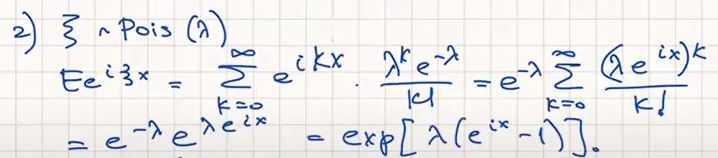
\includegraphics[]{images/pt1.JPG}
    \item $\xi \sim U[a, b]$, тогда $\charac{\xi}{x} = \E e^{ix\xi} = \frac{1}{b - a}\int\limits_a^b e^{ixt}dt = \frac{e^{itb} - e^{ita}}{it(b - a)}$
    \item $\xi \sim \mathcal{N}(0, 1)$, тогда $\charac{\xi}{x} = \int\limits_\R \frac{1}{\sqrt{2\pi}} e^{itx - \frac{t^2}{2}} dt = \int\limits_\R \frac{1}{\sqrt{2\pi}} e^{-\frac{(t - ix)^2}{2} - \frac{x^2}{2}} dt = e^{-\frac{x^2}{2}}$
    \item $\xi \sim \mathcal{N}(a, \sigma^2) \Longrightarrow \frac{\xi - a}{\sigma} \sim \mathcal{N}(0, 1)$
    $$
    \charac{\frac{\xi - a}{\sigma}}{x} = \E e^{i\frac{\xi - a}{\sigma}x} = e^{-\frac{x^2}{2}} \Longrightarrow \charac{\frac{\xi}{\sigma}}{x} =e^{ia\frac{x}{\sigma} - \frac{x^2}{2}} \Longrightarrow \charac{\xi}{x} = \charac{\frac{\xi}{\sigma}}{\sigma x} = e^{iax - \frac{\sigma^2x^2}{2}}
    $$
\end{enumerate}

\begin{theorem}[О единственности]

Если $\charac{\xi}{x}, \charac{\eta}{x}$ - характеристические функции случайных векторов одинаковой размерности и $\forall x \in \R^n \ \charac{\xi}{x} = \charac{\eta}{x}$, то $\xi = \eta$ по распределению (то есть случайные векторы имеют одинаковое распределение)

\end{theorem}

\begin{theorem}[О независимости]

$\xi_1, \ldots, \xi_n$ независимы $\Longleftrightarrow$ $\charac{(\xi_1, \ldots, \xi_n)}{x_1, \ldots, x_n} = \prod\limits_{j = 1}^n \charac{\xi_j}{x_j}$

\end{theorem}

\begin{proof} 
$\Longrightarrow$ 
$\xi_1, \ldots, \xi_n$ независимы, а значит и $(\cos(\xi_1x_1), \sin(\xi_1x_1)), \ldots, (\cos(\xi_nx_n), \sin(\xi_nx_n)))$ независимы. Тогда
\begin{multline*}
    \charac{(\xi_1, \ldots, \xi_n)}{x_1, \ldots, x_n} = \E e^{i(x_1\xi_1 + \ldots + x_x\xi_n)} = \E\brackets{\prod\limits_{j = 1}^n (\cos(\xi_jx_j) + i\sin(\xi_jx_j))} = \\
    = \prod\limits_{j = 1}^n\E\brackets{ \cos(\xi_jx_j) + i\sin(\xi_jx_j)} = \prod\limits_{j = 1}^n \E e^{ix_j\xi_j} = \prod\limits_{j = 1}^n \charac{\xi_j}{x_j}
\end{multline*}

$\Longleftarrow$
Рассмотрим $\eta = (\eta_1, \ldots, \eta_n)$ такие, что компоненты вектора независимы и $\forall j \leqslant n \ \xi_j = \eta_j$ по распределению.

Тогда $\charac{\eta}{x_1, \ldots, x_n} = \prod\limits_{j = 1}^n \charac{\eta_j}{x_j} = \prod\limits_{j = 1}^n \charac{\xi_j}{x_j} = \charac{(\xi_1, \ldots, \xi_n)}{x_1, \ldots, x_n}$. Значит по теореме о единственности $\eta = (\xi_1, \ldots, \xi_n)$ по распределению, а значит $\xi_1, \ldots, \xi_n$ независимы в совокупности. Вопрос: почему существует такое $\eta$\end{proof}

\paragraph*{Свертка}
\begin{statement}
$\eta, \xi$ независимы $\implies \varphi_{\xi + \eta}(x) = \varphi_{\xi}(x)\varphi_{\eta}(x)$
\end{statement}

\begin{proof} $\varphi_{\xi + \eta}(x) = \E e^{i(\xi + \eta)x} = \E e^{i\xi x} e^{i \eta x}= \E e^{i\xi x} \E e^{i \eta x} = \varphi_{\xi}(x)\varphi_{\eta}(x)$ \end{proof}
\bigskip

\begin{statement}
$\implies \varphi_{a\xi + b}(x) = e^{ibx} \varphi_{\xi}(ax)$
\end{statement}

\begin{proof} $\varphi_{a\xi + b}(x) = \E e^{i(a\xi + b)x} = \E e^{ia\xi x} e^{i bx}= e^{i bx} \E e^{i\xi ax} = e^{ibx} \varphi_{\xi}(ax)$ \end{proof}

\section{Четыре свойства характеристических функций с доказательством. Теорема об обращении (без доказательства). Теорема Бохнера–Хинчина.}
\paragraph*{Четыре свойства характеристических функций с доказательством}

\begin{enumerate}
    \item $|\charac{\xi}{t}| \leqslant \charac{\xi}{0} = 1$
    
    \begin{proof} $|\charac{\xi}{t}| = |\E e^{it\xi}| \leqslant \E|e^{it\xi}| = \E(1) = 1 = \charac{\xi}{0}$\end{proof}
    
    \item $\charac{\xi}{t}$ равномерно непрерывна на $\R$
    
    \begin{proof} Пусть $\eps > 0$. Так как $\sin(t\xi) \to 0$ почти наверное при $t \to 0$, по теореме Лебега о мажорируемой сходимости $\E|\sin(t\xi)| \to 0$ при $t \to 0$
    $$
    \exists \delta > 0: \forall t \in (-\delta, \delta) \ \E|\sin(t\xi)| < \frac{\eps}{4}
    $$
    Пусть $|s - t| < \delta$, тогда
    
   $|\charac{\xi}{t} - \charac{\xi}{s}| = |\E e^{is\xi}\brackets{e^{i(t - s)\xi} - 1}| \leqslant \E|e^{i(t - s)\xi} - 1| =$ \\ $ \E\sqrt{(\cos((t - s)\xi) - 1)^2 + \sin^2((t - s)\xi)} =
 \E\sqrt{2 - 2\cos((t - s)\xi)} = 2\E\Biggl|\sin\brackets{\frac{t - s}{2}\xi}\Biggr| < \eps
    $ \ \end{proof}
    
    \item $\forall t \in \R \ \charac{\xi}{t} \in \R \Longleftrightarrow \xi = -\xi$ по распределению.
    
    \begin{proof} 
    $\Longrightarrow$ 
    $\forall t \in \R \ \charac{\xi}{t} \in \R$, тогда
    $$
    \charac{\xi}{t} = \E e^{it\xi} = \E \brackets{\cos(t\xi) + i\sin(t\xi)} = \E \brackets{\cos(t\xi)} = \E \brackets{\cos(t\xi) - i\sin(t\xi)} = \charac{\xi}{-t}
    $$
    
    $\Longleftarrow$
    $\xi = -\xi$ по распределению, тогда $\E\sin(t\xi) = \E\sin(-t\xi) = -\E\sin(t\xi) = 0, \varphi_\xi(t) = \E\cos(t\xi)$  \end{proof}
     
    \item $\forall t \in \R \ \charac{\xi}{-t} = \overline{\charac{\xi}{t}}$
    
    \begin{proof} $\charac{\xi}{-t} = \E\brackets{\cos(-t\xi) + i\sin(-t\xi)} = \E\brackets{\cos(t\xi) - i\sin(t\xi)} = \E \overline{e^{it\xi}}  =\overline{\charac{\xi}{t}}$  \end{proof}
\end{enumerate}

\begin{theorem}[Об обращении (б/д)]  Пусть $\charac{\xi}{x}$ - характеристическая функция $\xi$. \end{theorem} 

\begin{itemize}
    \item Для любых двух точек непрерывности $a < b$ функции распределения $F_\xi$ верно, что  
    $$
    F_\xi(b) - F_\xi(a) = \frac{1}{2\pi}\lim\limits_{c \to \infty}\int\limits_{-c}^c \frac{e^{-ita} - e^{-itb}}{it} \charac{\xi}{t}dt
    $$
    \item Если $\int\limits_\R |\charac{\xi}{t}| dt < \infty$, то $\xi$-абс. непр. с $p_\xi(x) = \frac{1}{2\pi} \int\limits_\R e^{-itx} \charac{\xi}{t} dt$
\end{itemize}

\begin{lemmanote} 

Обратим внимание, что формулы выше по сути являются преобразованием Фурье (либо прямым, либо обратным).

\end{lemmanote} 

\paragraph*{Теорема Бохнера-Хинчина}

\begin{definition}  $\varphi: \R \to \mathbb{C}$ неотрицательно определена, если 
$$
\forall n \in \N \ \ \forall t_1, \ldots, t_n \in \R \ \  \forall z_1, \ldots, z_n \in \mathbb{C} \sum\limits_{j, k = 1}^n \varphi(t_j - t_k)z_j\overline{z_k} \geqslant 0
$$ \end{definition} 

\begin{theorem}[Бохнера-Хинчина]  

Если $\varphi$ непрерывна и $\varphi(0) = 1$, то 
\[\varphi - \text{хар. функция} \Leftrightarrow \varphi \text{ неотрицательно определена.}\] 

\end{theorem} 

\begin{proof} 
$\Longleftarrow$ Без доказательства

$\Longrightarrow$ Пусть $\varphi$ - характеристическая, тогда

$   \sum\limits_{j, k = 1}^n \varphi(t_j - t_k)z_j\overline{z_k} = \sum\limits_{j, k = 1}^n \E e^{i(t_j - t_k)\xi}z_j\overline{z_k} = \sum\limits_{j, k = 1}^n \E \brackets{e^{it_j\xi} \cdot \overline{e^{it_k\xi}}}z_j\overline{z_k} =$ \\
    $= \E\brackets{\sum\limits_{j, k = 1}^n z_j e^{it_j\xi} \cdot \overline{z_k e^{it_k\xi}}} = \E\Biggl|\sum\limits_{j = 1}^n z_k e^{it_k\xi}\Biggr|^2 \geqslant 0
$
\end{proof}
\section{Теорема о разложении характеристической функции в ряд (без доказательства). Теорема о непрерывности (без доказательства). Центральная предельная теорема.}
\begin{theorem}[О разложении характеристической функции в ряд (б/д)]
\hfill \break
\begin{enumerate}
    \item Пусть $\E|\xi|^n < \infty$, тогда $\forall r \leqslant n \ \exists \varphi^{(r)}_\xi(t) = \int\limits_{\R} (ix)^r e^{itx} dF_\xi(x), \ \ \E\xi^r = \frac{\varphi^{(r)}_\xi(0)}{i^r}$
    $$
    \charac{\xi}{t} = \sum\limits_{r = 0}^n \frac{(it)^r}{r!}\E\xi^r + \frac{(it)^n}{n!}\eps_n(t)
    $$
    
    Где $|\eps_n(t)| \leqslant 3\E|\xi|^n$ и $\lim\limits_{t \to 0}\eps_n(t) = 0$.
    
    \item Пусть  $\exists \varphi^{(2n)}(0) < \infty$, тогда $\E\xi^{2n} < \infty$ 
\end{enumerate}

\end{theorem}

\Example $\varphi(t) = e^{-t^4}$. Может ли она быть характеристической?

\Solution $\varphi^{'}(0) = 0, \ \varphi^{''}(0) = 0$, тогда по теореме выше существуют $\E\xi^2$ и $\E\xi$. Тогда $\E\xi^2 = \E\xi = 0 \Longrightarrow \xi = 0$ почти наверное, но при этом $\varphi_{\xi} \equiv 1$. Значит не может быть.

\begin{theorem}[О непрерывности (б/д)]
\hfill \break
\begin{itemize}
    \item Если $\xi_n \xrightarrow[]{d}  \xi$, то $\forall t \in \R \ \ \charac{\xi_n}{t} \to \charac{\xi}{t}$
    \item Если $\charac{\xi_n}{t}$~--- характеристические функции $\xi_n$, $\forall t \in \R \ \  \varphi_{\xi_n}(t) \to \varphi$ и $\varphi(t)$ непрерывна в 0, тогда $\xi_n \xrightarrow[]{d}  \xi$ для некоторой $\xi$ с характ. функцией $\varphi$  \\ (для случ. векторов $\xi_n \xrightarrow[]{d}  \xi \iff \varphi_{\xi_n}(t) \to \varphi(t) \ \forall x \in \R^k$)
\end{itemize}

\end{theorem}

\begin{theorem}[Центральная предельная теорема] 
Пусть $\xi_1, \xi_2, \ldots$~--- н.о.р.с.в. такие, что $\E\xi = a$, $\D\xi = \sigma^2$,  $S_n = \xi_1 + \ldots + \xi_n$. Тогда имеется сходимость по распределению

$$
\frac{S_n - na}{\sqrt{n\sigma^2}} \xrightarrow[]{d} \eta \sim \mathcal{N}(0, 1)
$$

\end{theorem}

\begin{lemmanote} 

В общей формулировке условия независимости и одинаковой распределенности не обязательны~--- можно ослабить.

\end{lemmanote}

\begin{lemmanote} 

В числителе $na =\E S_n, \sqrt{n\sigma^2} = \D S_n$; если дисперсия величин равна нулю, то это константы.

\end{lemmanote}

\begin{lemmanote} 

Идея: ЦПТ позволяет говорить о том, насколько точен закон больших чисел: на величину какого порядка (корень из дисперсии) мы можем отклоняться, когда делаем много опытов).

\end{lemmanote}

\begin{proof} Пусть $\widetilde{\xi_j} = \frac{\xi_j - a}{\sqrt{\sigma^2}}$. 
Тогда заметим, что $$\E\widetilde{\xi} = 0, \ \D\widetilde{\xi} = 1, \ \frac{S_n - na}{\sqrt{n\sigma^2}} = \frac{\widetilde{S}_n}{\sqrt{n}}$$
$$
    \charac{\frac{S_n - na}{\sqrt{n\sigma^2}}}{x} = \E e^{i \frac{\widetilde{S}_n}{\sqrt{n}} x} = \prod\limits_{j = 1}^n \charac{\widetilde{\xi_j}}{\frac{x}{\sqrt{n}}} = \brackets{\charac{\widetilde{\xi_1}}{\frac{x}{\sqrt{n}}}}^n = \ldots$$
    
По теор. о разложении в ряд для $n=2$ 
$$\varphi_\xi(t) = 1+it\E\xi - \frac{t^2}{2}\E\xi^2 + o(t^2)$$
$$\E\widetilde{\xi_1}=0,\ \E\widetilde{\xi_1}^2 = \D\widetilde{\xi_1} + (\E\widetilde{\xi_1})^2 = 1$$
$$\varphi_{\widetilde{\xi_1}} = 1 - \frac{t^2}{2} + o(t^2)$$

$$\ldots= \brackets{1 - \frac{1}{2}\brackets{\frac{x}{\sqrt{n}}}^2 + o\brackets{\frac{x^2}{n}}}^n =$$ 
$$ = exp\Big(n \ ln({1 - \frac{1}{2}\brackets{\frac{x}{\sqrt{n}}}^2 + o\brackets{\frac{x^2}{n}}}\Big) = $$
$$= exp\Big(n \Big(-\frac{x^2}{2n} + o\brackets{\frac{x^2}{n}}\Big) \Big) = e^{-\frac{x^2}{2} + o(1)} \to e^{-\frac{x^2}{2}}
$$

Тогда по теореме о непрерывности и о единственности получаем требуемое, так как предел характеристической функций совпадет с характеристической функцией стандартного нормального распределения. \end{proof}

\section{Гауссовские векторы. Три эквивалентных определения. Параметры распределения. Критерий независимости.}
\begin{definition} Случайный вектор $\xi = (\xi_1, \ldots, \xi_n)$ \textbf{гауссовский}, если $\charac{\xi}{y} = e^{i(a,\  y) - \frac{1}{2} (\Sigma\cdot y, \  y)}$, где $a \in \R^n$, $\Sigma$~--- симметричная неотрицательно определенная матрица, $(a, y)$ - скалярное произведение, иногда будем обозначать как $<a, y>$
\end{definition}

\begin{theorem}[Об эквивалентных определениях] Следующие утверждения эквивалентны:
\begin{enumerate}
    \item $\xi = (\xi_1, \ldots, \xi_n)$ гауссовский
    \item $\exists \eta_1, \ldots, \eta_m \sim \mathcal{N}(0, 1)$ независимые, $A \text{-матрица размера } {n \times m}$ и вектор $b \in \R^n$ такие что $\xi = A(\eta_1, \ldots, \eta_m)^T + b$
    \item $\forall \lambda \in \R^n$ $(\lambda, \xi) \sim \mathcal{N}(a, \sigma^2)$
\end{enumerate}
\end{theorem}
Из этой теоремы, в частности, следует, что матрица $\Sigma$ в определении гауссовского вектора является матрицей ковариаций этого вектора, а вектор $a$ — вектором математических ожиданий.

\begin{proof} 
$(1) \Longrightarrow (2)$

Будем считать, что $\Sigma$ невырождена как это было в лекциях.

Факт из линала: $(x, y) = x^Ty$

Пусть $|\Sigma| > 0$ и $\Sigma = C^TDC$, где $C$ ортонональная, а $D$ диагональная, тогда $D$ содержит на диагонали только положительные числа. Тогда $\Sigma = \brackets{\sqrt{D}C}^T E \sqrt{D}C$, где $E$ единичная. Поэтому 
$$
\charac{\xi - a}{x} = \E e^{i(\xi - a, x)} = e^{-i(a, x)}\charac{\xi}{x} =  e^{-\frac{1}{2} <\brackets{\sqrt{D}C}^T E\sqrt{D}Cx,\ x>} = e^{-\frac{1}{2} \brackets{\sqrt{D}Cx}^T \sqrt{D} Cx} 
$$

Тогда (с учетом того, что $C^{-1} = C^T$)
\begin{multline*}
    \charac{\brackets{\sqrt{D}}^{-1}C(\xi - a)}{x} = \E e^{i<\sqrt{D}^{-1}C(\xi - a), \  x>} = \E e^{i\brackets{\sqrt{D}^{-1}C(\xi - a)}^T x} = \E e^{i(\xi - a)^T C^T\sqrt{D}^{-1}x} = \\ = \E e^{i<\xi - a,\ (\sqrt{D}C)^{-1}x>}
    = \charac{\xi - a}{\brackets{\sqrt{D}C}^{-1}x} = e^{-\frac{1}{2}x^Tx}
\end{multline*}

Тогда заметим, что это характеристическая функция вектора, составленного из стандартных нормальных величин, при этом параметры из условия теоремы получились следующими: $\eta = \sqrt{D}^{-1}C(\xi - a)$, $A = C^T\sqrt{D}$, $b = a$.

$(2) \Longrightarrow (3)$

Пусть $\lambda = (\lambda_1, \ldots, \lambda_n)^T$, тогда 
$$
(\lambda, \xi) = \lambda^T(A\eta + b) = \sum\limits_{j = 1}^n \lambda_j \brackets{\sum\limits_{k = 1}^m a_{jk}\eta_k + b_j} = \sum\limits_{k = 1}^m c_k\eta_k + (\lambda, b)
$$

Где $c_k = \sum\limits_{j = 1}^n \lambda_ja_{jk}$, тогда $(\lambda, \xi) \sim \mathcal{N}\brackets{(\lambda, b), \sum\limits_{k = 1}^m c_k^2}$

$(3) \Longrightarrow (1)$

$$
\charac{\xi}{\lambda} = \E e^{i(\lambda, \xi)} = \charac{(\lambda, \xi)}{1} = e^{i\E(\lambda, \xi) - \frac{1}{2}\D(\lambda, \xi)} = e^{i(\lambda, a) - \frac{1}{2}\sum\limits_{j, k = 1}^n\lambda_i\lambda_j cov(\xi_j, \xi_k)} = e^{i(\lambda, a) - \frac{1}{2}(\Sigma\lambda, \lambda)}
$$

Таким образом, мы получили, что $a$~--- вектор математических ожиданий, а $\Sigma$~--- матрица ковариаций. Ее симметричность по определению. Неотрицательность докажем по определению:

$
\lambda^T\Sigma\lambda = \sum\limits_{j, k = 1}^n \lambda_j\lambda_k cov(\xi_j, \xi_k) = \D\brackets{\sum\limits_{j = 1}^n \lambda_j\xi_j} \geqslant 0
$\end{proof}

\begin{corollary}[Параметры распределения] В определении гауссовского вектора $a$~--- вектор математических ожиданий, а $\Sigma$~--- матрица ковариаций, то есть $\xi \sim \mathcal{N}(a, \Sigma)$
\end{corollary}

\begin{theorem}[Критерий независимости] Компоненты $\xi = (\xi_1, \ldots, \xi_n)$ - гауссовского вектора независимы $\iff$ их ковариации равны 0
\end{theorem}

\begin{proof} В правую сторону очевидно. Докажем в обратную. Пусть $\forall i \neq j \ cov(\xi_i, \xi_j) = 0$, тогда матрица $\Sigma$ будет иметь диагональный вид, где на диагонали будут стоять $\D\xi_i \implies \varphi_\xi(x) = e^{i<\E\xi, \ x> - \frac{1}{2}\sum\limits_{j=1}^n(\D\xi_j)x_j^2} = \prod\limits_{j=1}^n e^{i<\E\xi_j, \ x_j> - \frac{1}{2}(\D\xi_j)x_j^2} = \prod\limits_{j=1}^n \varphi_{\xi_j}(x_j)$ \end{proof}

\section{Сходимости векторов.Связь между сходимостью векторов и покомпонентной сходимостью. Законы больших чисел. Многомерная центральная предельная теорема (б/д).}
\begin{definition} Последовательность случайных векторов $\xi_k$ сходится почти наверное к $\xi$, если 
$P(\{ \omega| \ \xi_n(\omega) \to \xi(\omega) \} )= 1$
\end{definition}

\begin{definition} Последовательность случайных векторов $\xi_k$ сходится по вероятности к $\xi$, если 
$\forall \eps > 0\ P\brackets{\|\xi_k - \xi\|_2 \geqslant \eps} \to 0 \text{, где } \|x\|_2 = \sqrt{x_1^2 + \ldots + x_n^2}
$
\end{definition}

\begin{definition} Последовательность случайных векторов $\xi_k$ сходится в $L_p$ к $\xi$, если \newline
$
\E\brackets{\|\xi_k - \xi\|_p}^p \to 0 \text{, где } \|x\|_p = \brackets{|x_1|^p + \ldots + |x_n|^p}^{\frac{1}{p}}
$
\end{definition}

\begin{definition} Последовательность случайных векторов $\xi_k$ сходится по распределению к $\xi$, если $\forall f: \R^n \to \R$ ограниченной и непрерывной верно, что $\E f(\xi_k) \to \E f(\xi)$

(или $\forall B \in \mathcal{B}(\R^k): P_\xi(\partial B) = 0 \ P(\xi_n \in B) \to P(\xi \in B)$)
\end{definition}

\begin{theorem}[Связь между сходимостью векторов и покомпонентной сходимостью] Верно:
\begin{enumerate}
    \item $\xi_n \xrightarrow[]{\text{п.н.}}  \xi \iff \forall j \ \  \xi_n^j \xrightarrow[]{\text{п.н.}} \xi^j$
    \item  $\xi_n \xrightarrow[]{P}  \xi \iff \forall j \ \  \xi_n^j \xrightarrow[]{P} \xi^j$
    \item  $\xi_n \xrightarrow[]{L_p}  \xi \iff \forall j \ \  \xi_n^j \xrightarrow[]{L_p} \xi^j$
    \item  $\xi_n \xrightarrow[]{d}  \xi \implies \forall j \ \  \xi_n^j \xrightarrow[]{d} \xi^j$
\end{enumerate}
\end{theorem}

\begin{proof}
1. Очевидно \\
2. $\implies$ $\{ |\xi_n^j - \xi^j| > \eps\} \subset \{ \|\xi_n - \xi\|_2 > \eps\}$, \ \  $P(\{ \|\xi_n - \xi\|_2 > \eps\}) \to 0 \implies P(\{ |\xi_n^j - \xi^j| > \eps\}) \to 0$\\
$\impliedby$ $\{ \|\xi_n - \xi\|_2 > \eps\} \subset \bigcup\limits_{j = 1}^k \{ |\xi_n^j - \xi^j| > \frac{\eps}{k}\}, \ \ P(\{ \|\xi_n - \xi\|_2 > \eps\}) \leqslant \sum\limits_{j = 1}^k P(\{ |\xi_n^j - \xi^j| > \frac{\eps}{k}\}) \to 0$\\
3. $\implies$ $\E|\xi_n^j - \xi^j|^p \leqslant  \sum\limits_{j = 1}^k \E|\xi_n^j - \xi^j|^p = \E\brackets{\|\xi_k - \xi\|_p}^p \to 0 $ \\
$\impliedby$ $\E\brackets{\|\xi_k - \xi\|_p}^p = \sum\limits_{j = 1}^k \E|\xi_n^j - \xi^j|^p \to 0$\\
4. $\implies$ т.к. выполненно для любой функции, то возьмем $f_i(x_1, \ldots, x_n) = x_i$, то есть $\forall i \ \ \E f_i(\xi_k) = \E \xi_k^i \to \E f_i(\xi) = \E \xi^i$, то есть $\forall i \ \ \xi_n^j \xrightarrow[]{d} \xi^j$
\end{proof}

\textbf{Контрпример для сходимости по распределению:} $\xi, \eta$ - н.о.р.с.в., $\xi_n \xrightarrow[]{d} \xi, \eta_n \xrightarrow[]{d} \eta \stackrel{d}{=} \xi$, но $(\xi_n, \eta_n) \stackrel{d}{\nrightarrow} (\xi, \xi)$, а $(\xi_n, \eta_n) \xrightarrow[]{d} (\xi, \eta)$

\begin{theorem}
\begin{enumerate}
    \item Из сходимости почти наверное следует сходимость по вероятности
    \item Из сходимости по вероятности следует сходимость по распределению
    \item Из сходимости в $L_p$ следует сходимость по вероятности
\end{enumerate}
\end{theorem}


\begin{theorem}[Закон больших чисел]
Пусть $\xi_1, \xi_2, \ldots$~--- попарно независимые случайные векторы, дисперсия каждого ограничена константой $C$, тогда $\forall w(n) \to +\infty$ имеется следующая сходимость по вероятности:
$$
\frac{S_n - \E S_n}{\sqrt{n}w(n)} \xrightarrow[]{P} 0
$$
\end{theorem}

\begin{proof} Заметим, что для каждой координаты это верно (доказано выше), а покоординатная сходимость по вероятности эквивалентна сходимости всего вектора по вероятности. \end{proof}

\begin{theorem}[УЗБЧ]

Пусть $\xi_1, \xi_2, \ldots$~--- н.о.р.с. векторы, при этом $\E\xi_i = 0$. Имеется следующая сходимость почти наверное:
$$
\frac{\xi_1 + \ldots + \xi_n}{n} \xrightarrow[]{\text{п.н.}}  0
$$
\end{theorem}

\begin{proof} Заметим, что для каждой координаты это верно (доказано выше), а покоординатная сходимость почти наверное эквивалентна сходимости всего вектора почти наверное.\end{proof}

\begin{lemma} $\xi_k \to \xi$ по распределению тогда и только тогда, когда $\forall y \in \R^n \ \charac{\xi_k}{y} \to \charac{\xi}{y}$
\end{lemma}

\begin{theorem}[Многомерная центральная предельная теорема (б/д)] Пусть $\xi_1, \xi_2, \ldots$~--- н.о.р.с. векторы, $\E\xi_i = a$ матрица ковариаций $\Sigma$, тогда верна сходимость по распределению:
$$
\frac{S_n - na}{\sqrt{n}} \xrightarrow[]{d} \eta \sim \mathcal{N}(0, \Sigma)
$$
\end{theorem}
\end{document}
